%==============================================================================
% SIMTiX v2 --- IEEE Transactions on VLSI Systems manuscript (journal format).
% Build:  pdflatex simtix_tvlsi && pdflatex simtix_tvlsi
% Figures: docs/plot_vortex.py, docs/plot_lanes.py (into docs/figs/).
% \tbd{...} marks numbers still to be measured (none at present).
% Supplementary material: simtix_tvlsi_supp.tex (build after this file).
%==============================================================================
\documentclass[journal]{IEEEtran}

\usepackage{cite}
\usepackage{amsmath,amssymb}
\usepackage{graphicx}
\usepackage{booktabs}
\usepackage{multirow}
\usepackage{array}
\usepackage{xcolor}
\usepackage{tikz}
\usetikzlibrary{positioning,fit,backgrounds,arrows.meta,calc}
\usepackage{url}
\usepackage[hidelinks]{hyperref}

\graphicspath{{../figs/}}
\newtheorem{theorem}{Theorem}
\newtheorem{proposition}{Proposition}
\newtheorem{corollary}{Corollary}
\setlength{\tabcolsep}{3.5pt}
\renewcommand{\arraystretch}{1.08}
\newcommand{\Fmax}{$F_{\max}$}
\newcommand{\tbd}[1]{\textcolor{red}{[#1]}}

\begin{document}

\title{SIMTiX: A Compact RISC-V SIMT Accelerator With Line-Aggregated Atomic
Operations for FPGA Systems-on-Chip}

\author{Krishna~Gorai and Bikram~Paul%
\thanks{K. Gorai and B. Paul are with the School of Computing and Electrical
Engineering, Indian Institute of Technology Mandi, Mandi 175075, India (e-mail:
kg05112001@gmail.com; bikram@iitmandi.ac.in).}}

\markboth{IEEE Transactions on Very Large Scale Integration (VLSI) Systems}%
{Gorai and Paul: SIMTiX: A Compact RISC-V SIMT Accelerator}

\maketitle

\begin{abstract}
This paper presents SIMTiX, a RISC-V single-instruction multiple-thread (SIMT)
accelerator for FPGA systems-on-chip, and explains its performance against three
RISC-V machines of other organizations on the same board. SIMTiX has eight lanes and
eight warps, FP32/FP16 arithmetic, warp shuffles, block barriers and RV32A atomic
memory operations (AMOs). Its two-stage issue logic lets a warp sleep while its
operands are pending, so that few warps hide the latency of the functional units and
of memory, and per-warp memory contexts, a line coalescer and a non-blocking 64~KB L1
keep up to 16 line requests in flight to the DDR4 of a Zynq UltraScale+.
Line-aggregated AMOs serve all lanes of an AMO that fall in one cache line with one
read and one write and return the values of serial execution; they speed up a
histogram by $2.47\times$ for 660 lookup tables (LUTs). The complete board design uses
107,658 LUTs and closes at 115.4~MHz on the ZCU102. A 16-lane version, whose store
logic we restructure from 37,450 to 11,047 LUTs, closes at 100~MHz and runs 82
benchmark runs $1.45\times$ faster than the eight-lane design. On 15 Rodinia and RiVEC
benchmarks, SIMTiX is $16.9\times$, $3.1\times$ and $2.5\times$ faster than the scalar
core CVA6, the vector processor Ara and the SIMT GPGPU Vortex, each built for the same
board (geometric means). We split each ratio into clock, peak width and efficiency.
Against Ara, SIMTiX's lead per cycle is its width; its efficiency is 2.4 to 17 times
higher on gathers and reductions but lower on unit-stride streams. Against Vortex, of
equal width, the whole factor of 2.7 is efficiency.
\end{abstract}

\begin{IEEEkeywords}
Atomic memory operations, FPGA, general-purpose GPU (GPGPU), RISC-V,
single-instruction multiple-thread (SIMT), soft processor.
\end{IEEEkeywords}

%==============================================================================
\section{Introduction}
%==============================================================================
\IEEEPARstart{F}{ield}-programmable gate array (FPGA) systems-on-chip such as the
AMD Zynq UltraScale+ combine hard processor cores with programmable logic.
Typically the processors run the control code and the logic holds fixed-function
accelerators, each synthesized for one kernel. A programmable data-parallel
engine in the logic can instead serve many kernels without a new bitstream.
Graphics processing units (GPUs) provide such an engine through the
single-instruction multiple-thread (SIMT) model: scalar threads are grouped into
warps that execute one instruction stream on a vector of lanes, and the hardware
switches between warps to hide memory latency~\cite{tesla,aamodt}.

A number of soft GPUs have been published (Section~\ref{sec:related}). The
compact ones have no cache; eGPU~\cite{egpu}, for example, reaches global data
through its shared memory. The ones with a complete memory system, such as
Vortex~\cite{vortex} and Ventus~\cite{ventus25}, are large: one Ventus streaming
multiprocessor occupies 329k LUTs. The designs are also evaluated on different
devices, with different tools and benchmarks, so their costs cannot be compared
directly. A SIMT engine in the logic also competes with machines of other
organizations: scalar RISC-V cores such as CVA6~\cite{cva6}, and vector processors of
the RISC-V vector extension such as Ara~\cite{ara,ara2}. Which of these organizations
makes the best use of the logic of one device, and why, has not been measured on one
board with one set of benchmarks.

Atomic memory operations (AMOs) are a particular problem for a soft SIMT engine.
One AMO instruction of a warp of $L$ lanes is $L$ read-modify-write operations,
and in histogram, clustering and graph kernels many of them fall in the same
cache line or on the same word. A GPU executes them in atomic units at its L2
cache~\cite{fermi}. In an FPGA system-on-chip the accelerator reaches memory
through the AXI4 ports of the processing system, which have no atomic
transactions, so the accelerator must perform every AMO itself as a read and a
write. Performed one lane at a time, the atomics become the bottleneck of these
kernels.

SIMTiX is designed from the outset as a peripheral of the processing system: the
Cortex-A53 is the host, kernel data lives in DDR4, and the complete board design,
not only the accelerator, has to close timing. SIMTiX makes the following
contributions:
\begin{enumerate}
\item \emph{Latency tolerance with few warps}: a two-stage issue logic in which a
warp whose operands are pending sleeps behind a register scoreboard while the other
warps issue, with pipelined units and non-blocking loads. We bound the issue rate by
the distance between a warp's issues and measure the effect of each mechanism: together
they gain $1.68\times$ over our earlier design with the same instructions
(Section~\ref{sec:arch}).
\item \emph{Memory-level parallelism for the processing system's DDR4}: per-warp
memory contexts, a coalescer that sends one request per line touched, and a
non-blocking 64~KB L1 with 16 miss-status holding registers, which keep up to 16
line requests in flight, with two ordering rules for the AXI4 port that the board
showed to be necessary (Section~\ref{sec:l1}).
\item \emph{Line-aggregated AMOs}: all lanes of an AMO that fall in one line are
served with one read and one masked write, and every lane receives the value of
serial execution in lane order. We give a one-lane-per-cycle and a parallel
variant, with their cost and benefit (Sections~\ref{sec:amo}
and~\ref{sec:evalamo}).
\item \emph{A same-board comparison of four organizations}: SIMTiX, the scalar core
CVA6, the vector processor Ara and the SIMT GPGPU Vortex, each built for the ZCU102
and run on Rodinia, RiVEC and our applications with every output checked. We split
each time ratio into clock, peak width and efficiency, which attributes SIMTiX's
lead to the mechanisms above and identifies its limits
(Sections~\ref{sec:machines}--\ref{sec:decomp}).
\item \emph{Scaling to 16 lanes on the board}: a store-merging structure that shrinks
the 16-lane memory engine by 46\% at equal function, a divide/square-root
unit per eight lanes and an L1 that keeps its line count at no block-RAM cost. The
16-lane board design closes at 100~MHz, runs all benchmarks $1.45\times$ faster than
the eight-lane design, and matches the cycle ratios of its simulation with a median
error of 1\% (Section~\ref{sec:lanes16}).
\end{enumerate}
Our goal is not to compete with hard GPUs or with multi-core soft GPGPUs, but to
provide a compact programmable engine with a complete memory system beside the
host processor of a mid-size FPGA system-on-chip. The register-transfer-level
(RTL) source, kernels, testbenches, Vortex port and scripts are available at
\url{https://github.com/Krishna-Gorai/simtix}.

%==============================================================================
\section{Comparison to Other Soft GPU Architectures}\label{sec:related}
%==============================================================================
FlexGrip~\cite{flexgrip} executes CUDA binaries on an FPGA, and
FGPU~\cite{fgpu} is an OpenCL-programmed SIMT processor. MIAOW~\cite{miaow}
implements the AMD Southern Islands compute unit in RTL but models its memory
hierarchy in software. Nyami~\cite{nyuzi} is a synthesizable GPU model, and
Simty~\cite{simty} executes the RISC-V instruction set with a generalized SIMT
front end. eGPU~\cite{egpu} places 16 scalar processors and 512 threads in 5,600
Agilex logic modules and closes above 770~MHz. Vortex~\cite{vortex} extends
RISC-V with instructions for warp control, divergence and barriers, and provides
a configurable multi-core GPGPU with L1 and L2 caches, local memory and an OpenCL
stack. Ventus~\cite{ventus25} builds a GPGPU on the RISC-V vector extension; its
vector register file is 54\% of the area of a streaming multiprocessor.

Beside the GPU instruction sets compared in~\cite{vortex} (Table~SI of the
supplementary material), SIMTiX runs one scalar RV32 thread per lane, like
Vortex, but differs in three columns. It needs no thread-control or divergence
instructions: the hardware spawns the warps, \texttt{ecall} ends a warp, and the
reconvergence stack detects divergence from the branch outcomes and reconverges
without the split and join instructions that Vortex's compiler inserts. It has no
fence; a barrier releases only when the memory operations issued before it have
completed. And its GPU operations are a warp shuffle and an INT8 dot product
rather than texture sampling.

\begin{table}[t]
\caption{Resource Comparison}
\label{tab:soa}
\centering\footnotesize
\setlength{\tabcolsep}{2.4pt}
\begin{tabular}{lllrrr}
\toprule
Architecture & Device & Configuration & LUTs & DSP & \Fmax\\
\midrule
FGPU~\cite{fgpu}$^a$         & Xilinx 28~nm & 2 CU $\times$ 8 PE & 57k & 48 & 250\\
FlexGrip~\cite{flexgrip}$^a$ & Xilinx 40~nm & 1 SM $\times$ 16 PE & 100k & 300 & 100\\
eGPU~\cite{egpu}             & Agilex & 1 SM $\times$ 16 SP & 5.6k$^b$ & 24 & 771\\
Ventus~\cite{ventus25}       & VU37P & 1 SM & 329k & --- & ---\\
Vortex~\cite{vortex}$^c$     & XCZU7EV & 4 warps $\times$ 8 & 80.1k & 48 & 140.8\\
SIMTiX$^c$                   & XCZU7EV & 4 warps $\times$ 8 & 84.4k & 72 & 101.6\\
\bottomrule
\end{tabular}

\vspace{2pt}
\begin{minipage}{\columnwidth}\footnotesize
$^a$As reported in~\cite{egpu}. $^b$Adaptive logic modules. $^c$Built in this
work with the same flow (Section~\ref{sec:method}). CU: compute unit; PE:
processing element; SM: streaming multiprocessor; SP: scalar processor. \Fmax\
in MHz.
\end{minipage}
\end{table}

Table~\ref{tab:soa} compares the resources of these designs, counted in lookup
tables (LUTs) and digital signal processing (DSP) blocks. This comparison is only
representative: the devices, tools and configurations differ, and the
frequencies of the earlier designs are taken from their papers. One Ventus
streaming multiprocessor needs more LUTs than the 230,400 of our device, so it
cannot be built for it. SIMTiX is closest to Vortex: both execute one scalar
RISC-V thread per lane with a few custom instructions, and Vortex can be
configured with the same warp and lane counts. We therefore built Vortex~3.0 for
our device with our flow and compare the two directly in
Section~\ref{sec:evalvortex}.

GPUs execute global atomics in atomic units at the L2 cache~\cite{fermi}, and in
the GPU model of~\cite{dab} the atomics of a warp that fall in one cache sector
form one transaction. Franey and Lipasti studied hardware support for GPU
atomics~\cite{franey}. PHI buffers and coalesces commutative updates in the
caches of a multicore~\cite{phi}, and DAB buffers GPU atomics to make them
deterministic~\cite{dab}. In software, warp-aggregated atomics combine the
same-address increments of a warp with shuffles and let one elected lane perform
a single atomic~\cite{warpagg}; this needs a commutative operation on one address
and a change to the kernel. Vortex~3.0 sends the AMO of each lane as a separate
request to a bank of its last-level cache, which reads, modifies and writes one
word per request. SIMTiX aggregates in the memory engine of the core, ahead of the
L1. The aggregation covers lanes on different words of one line and lanes on the
same word, applies to every RV32A AMO including swap, minimum and maximum, returns
the old value of every lane, and needs no change to the kernel.

%==============================================================================
\section{Architecture}\label{sec:arch}
%==============================================================================
\begin{figure*}[t]
\centering
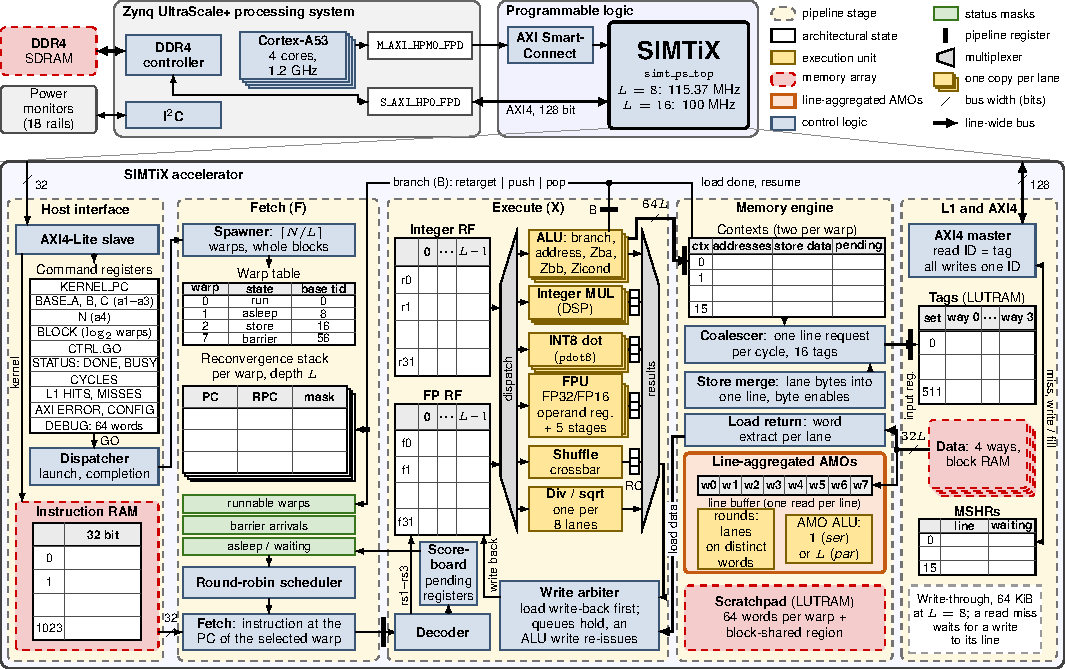
\includegraphics[width=\textwidth]{simtix_arch_v3.pdf}
\caption{SIMTiX on the ZCU102 (top) and the accelerator by pipeline stage
(bottom). The Cortex-A53 writes the kernel and the launch parameters over
AXI4-Lite and polls for completion. The scheduler selects a runnable warp, whose
instruction is fetched (F) at the top of its reconvergence stack, decoded and
executed (X) on the eight lanes or issued to a multi-cycle unit; the register
scoreboard holds back an instruction whose operands are still in flight, and the
warp sleeps until one of its results is written. Branch outcomes update the stack
one cycle after execution (B). A memory instruction passes to a context of its
warp, which coalesces it into line requests and executes AMOs one line at a time.
Line requests reach DDR4 through the L1 data cache, the AXI4 master and the port
S\_AXI\_HP0. The register files, the L1 tags and the scratchpad are in LUTRAM.
RF: register file; tid: thread ID; RPC: reconvergence PC; MSHR: miss-status
holding register.}
\label{fig:arch}
\end{figure*}

SIMTiX is organized in a typical SIMT machine topology, but is designed from the
start as a peripheral of an FPGA system-on-chip. A kernel is launched for $N$
threads. We will use the term \emph{warp} to denote $L$ threads that execute one
instruction together, one per \emph{lane}, and \emph{block} to denote a group of
$2^b$ warps that can synchronize at a barrier and share a scratchpad. $W$ warps are
resident at a time; the board design has $W=8$ and $L=8$. Fig.~\ref{fig:arch}
shows the board system (top) and the accelerator grouped by pipeline stage
(bottom).

\subsection{System and Host Interface}
One Cortex-A53 core runs a bare-metal host program. It reaches the accelerator
through the PS master port M\_AXI\_HPM0\_FPD and an AXI SmartConnect, which
converts the transactions to AXI4-Lite. The \emph{AXI4-Lite slave} of the
accelerator decodes two windows. The first holds the \emph{command registers}:
the kernel PC, the address of the kernel's parameter block, the thread count $N$,
the block size and GO, and, for reading, DONE, the cycle count of the last
launch, the L1 read hits and misses, and a sticky AXI error flag. The second is
the \emph{instruction RAM}, 1,024 32-bit words, into which the host writes the
kernel. When the host writes GO, the \emph{dispatcher} invalidates the L1, starts
the warps, counts cycles until the last warp finishes, and sets DONE.

Kernel data lives in DDR4, which the accelerator reaches through its AXI4 master
and the 128-bit high-performance port S\_AXI\_HP0 of the processing system (PS).
This port is not coherent with the A53 caches, so the host cleans its data cache
before GO and invalidates it after DONE. The I$^2$C controller of the PS reads the
board's power monitors (Section~\ref{sec:evalboard}).

\subsection{Fetch Stage}
The \emph{spawner} divides the threads into $\lceil N/L\rceil$ warps and places
one per cycle into a free slot of the \emph{warp table}, so a slot is refilled as
soon as its warp finishes; the last warp is masked if $N$ is not a multiple of
$L$. A block is spawned whole into a group of $2^b$ slots, so its warps are always
resident together. The warp table holds the state of each slot and the thread ID
of its lane~0. A warp is running, asleep on the register scoreboard, waiting for
a store, AMO or the shared divide unit, at a barrier, or finished.

Each warp has a \emph{reconvergence stack}~\cite{fung,aamodt} whose frames hold a
PC, a reconvergence PC (RPC) and an active mask; the top frame gives the warp's PC
and the lanes that execute. A uniform branch only changes the PC of the top frame.
When the lanes of a warp disagree, the branch diverges: a forward branch pushes
the not-taken lanes with the branch target as RPC, and a backward branch (a loop)
pushes the lanes that stay in the loop with the fall-through PC as RPC. A frame
whose PC reaches its RPC is popped in an issue slot of its own, and the warp
continues with the lanes of the frame below. Jumps are uniform and only retarget the
top frame. These rules bound the depth of the stack.

\begin{theorem}\label{thm:stack}
Let a warp start with the non-empty set of active lanes $A_0\subseteq\{0,\dots,L-1\}$.
Its reconvergence stack never holds more than $|A_0|\le L$ frames, and a warp can
reach $|A_0|$ frames.
\end{theorem}
\begin{IEEEproof}
Number the frames from the bottom and let $A_j$ be the lane set of frame $j$. We show
that $\emptyset\neq A_{j+1}\subsetneq A_j$ holds for every pair of adjacent frames at
all times. It holds for the single initial frame. A uniform branch or a jump changes
only the PC of the top frame, and a pop removes the top frame; neither breaks the
chain below. A divergent branch of the top frame $k$, with taken lanes $T$, satisfies
$\emptyset\neq T\subsetneq A_k$ by the definition of divergence; it leaves $A_k$ in
frame $k$ and pushes either $A_k\setminus T$ (forward branch) or $T$ (backward
branch), and both are non-empty strict subsets of $A_k$. Hence the lane sets form a
strictly decreasing chain of non-empty subsets of $A_0$. Each step of the chain
removes at least one lane, so it has at most $|A_0|$ members. The bound is reached by
a loop that the lanes of $A_0$ leave at $|A_0|$ different iterations: each exit except
the last is a divergent backward branch that pushes the remaining lanes, one lane
fewer each time.
\end{IEEEproof}

We therefore set the depth to $L$. A depth below $L$ is unsafe for a reason other
than nesting: a single loop whose trip count differs per lane can use every frame
(Section~\ref{sec:evallanes}).

The \emph{status masks}, derived from the warp table, give the runnable warps, the
sleeping and waiting warps, and the warps at a barrier. A warp at \texttt{bar} waits until every
live warp of its block has arrived. The \emph{round-robin scheduler} selects the
next runnable warp after the one issued last, and the \emph{fetch} block reads the
instruction at the PC of its top frame into the pipeline register between the two
stages.

\subsection{Execute Stage}
The \emph{decoder} accepts RV32I, the RV32M \texttt{mul}, the RV32A AMOs without
load-reserved and store-conditional, and the single- and half-precision
floating-point instructions. Three custom instructions use the \emph{custom-0}
opcode space: \texttt{pdot8}, a dot product of four signed or unsigned 8-bit
integer (INT8) pairs; \texttt{shfl.\{idx,up,down,xor\}}; and \texttt{bar}. It
also accepts three small standard extensions that shorten the kernels' address
and selection code: from Zba the shift-and-add instructions
\texttt{sh\{1,2,3\}add}, which form an array element's address in one instruction;
from Zbb the integer \texttt{min}, \texttt{max}, \texttt{minu} and \texttt{maxu};
and from Zicond \texttt{czero.eqz} and \texttt{czero.nez}, which zero a register
under a condition and so select a value without a branch. They add a decode of
the full 7-bit function field and one result multiplexer per lane on the register
write path, not on the address path.

The integer \emph{register file} (RF) has two read ports and the floating-point RF
three, for the fused multiply-add (FMA). Both hold 32 registers per thread in
distributed RAM (LUTRAM), one bank per lane addressed by warp and register. We
moved the RFs from flip-flops to LUTRAM because a flip-flop RF needs a 128-to-1
multiplexer per lane and read port; this reduced the LUTs of the integer
accelerator from 170,868 to 30,088. A register not yet written in a launch reads
its initial value (the thread ID for \texttt{a0}, the launch arguments for
\texttt{a1}--\texttt{a4}, zero otherwise), so no cycles are spent clearing the RFs.

The \emph{dispatch} multiplexer sends the operands of the active lanes to the
selected unit. The \emph{ALU} of each lane executes the integer instructions,
evaluates branch conditions and computes memory addresses. A branch or jump
updates the reconvergence stack in a stage of its own one cycle after execution
(B in Fig.~\ref{fig:arch}), from its registered outcome; the warp is not fetched
again before then. All other units take more than one cycle and accept a new warp
instruction every cycle. Each carries the instruction's warp and destination
register down a delay line in step with its pipeline, and a \emph{result queue}
holds finished results until the register file's write port is free; a unit
holds at most eight instructions in its pipeline and queue together. A \emph{register scoreboard} marks, per warp, the integer and
floating-point registers whose values are still in a unit or its queue. The
issue stage holds back an instruction that reads or writes a marked register or
whose unit is full, and that warp then sleeps, without taking fetch slots from
the other warps, until one of its own results is written (or, if its unit was
full, any result). So a warp continues with independent instructions while its
multiply, FMA or shuffle results are pending.

\begin{figure*}[t]
\centering
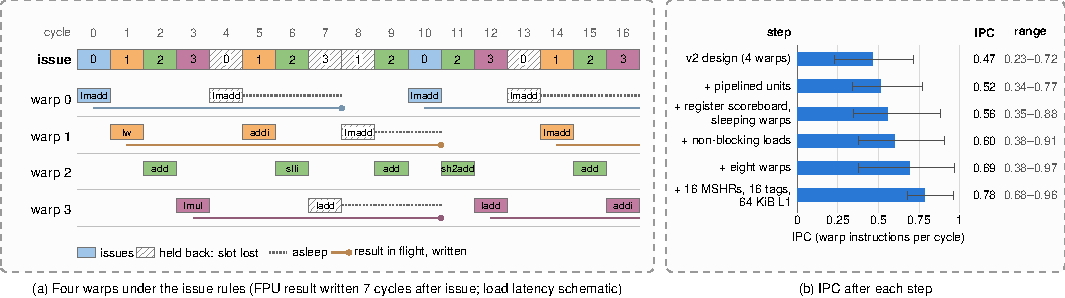
\includegraphics[width=\textwidth]{simtix_lat.pdf}
\caption{Latency tolerance in the issue stage. (a) Four warps under the issue rules of
SIMTiX: one warp instruction per cycle, chosen round robin among the runnable warps; a
warp at most every other cycle; a warp whose source register is pending sleeps until
the result is written; a load does not stop its warp. The FPU result is written six
cycles after issue; the load latency is schematic. With four warps, three issue slots
stay empty. (b) Measured speed-up of the mechanisms over the v2 design, added one at a
time, with the board's application inputs and an AXI4 memory model of 24 cycles:
geometric mean and range over eight applications, and the IPC. The instruction count
is the same in every step, so every gain comes from hiding latency.}
\label{fig:lat}
\end{figure*}

These rules bound the issue rate. Let $d_w$ be the mean distance, in cycles, between
consecutive issues of warp $w$ when it runs alone, and IPC the warp instructions
issued per cycle.

\begin{proposition}\label{prop:ipc}
$W$ warps sharing the issue slot reach
\begin{equation}
\mathrm{IPC}\le\min\Bigl(1,\ \sum_{w=1}^{W}\frac{1}{d_w}\Bigr),
\label{eq:ipc}
\end{equation}
with $d_w\ge2$ for every warp and $d_w\ge7$ in a chain of dependent FMAs. Warps of
equal distance $d$ need $W\ge d$ to issue in every cycle.
\end{proposition}
\begin{IEEEproof}
There is one issue slot per cycle, so $\mathrm{IPC}\le1$. A warp's own constraints
are the fetch-issue sequence, which keeps it from being fetched while its previous
instruction is in X, and the waits for its own results. Other warps cannot shorten
either; they can only delay its fetch or, through the shared write ports, its result
writes. So in any interval of $T$ cycles warp $w$ issues at most $T/d_w+1$
instructions, and the sum over the warps, divided by $T$, tends to the bound as $T$
grows. A warp fetched in cycle $t$ issues in $t+1$ and can be fetched again in $t+2$
at the earliest, so $d_w\ge2$. An FMA's result is written six cycles after issue, and
an instruction that reads it can issue in the next cycle at the earliest, so a chain
of dependent FMAs has $d_w\ge7$. With $d_w=d$ for all $w$, the bound reaches 1 only
if $W/d\ge1$.
\end{IEEEproof}

So two warps can fill the issue slot with independent integer code, and a chain of
dependent FMAs needs seven. Fig.~\ref{fig:lat}(a) shows the case $W=4$: while
warps 0 and 3 wait for the FPU, warps 1 and 2 issue, and the slot stays empty only
when all four wait. A deeper pipeline raises every $d_w$ and so needs more warps for
the same IPC; Vortex, whose FMA takes 16 cycles, reaches its highest IPC of the
configurations we built with 16 warps (Section~\ref{sec:evalvortex}). Fig.~\ref{fig:lat}(b) gives the measured effect
of each mechanism. Pipelining the units, so that each accepts a warp instruction every
cycle, gains $1.11\times$; the register scoreboard with sleeping warps $1.07\times$
more; non-blocking loads $1.08\times$; eight warps instead of four $1.15\times$; and
16 MSHRs with a 64~KB L1, which keep more misses in flight, $1.13\times$, for
$1.68\times$ together and an IPC that rises from 0.47 to 0.78.

Each lane has a
pipelined integer multiplier on DSP blocks, an INT8 dot-product unit, and an
FP32/FP16 unit (\emph{FPU}) for addition, multiplication, the four FMA variants,
comparisons, minimum and maximum, sign injection, conversions and
classification. The FPU has five pipeline stages, and its 48-bit significand
product is formed on a $24\times24$ cascade of DSP blocks. FP16 operations widen
their operands to FP32, use the FP32 datapath and round the result to FP16, so an
FP16 result is rounded twice. Let $\circ_p$ denote rounding to nearest even and
$\square_p$ rounding to odd, at $p$ bits of significand: 24 for FP32, 11 for FP16.

\begin{proposition}\label{prop:fp16}
Let $x$ be the exact sum, difference, product, quotient or square root of FP16
operands, and $y=ab+c$ the exact result of an FMA of FP16 operands, with results in
the normal range of FP16. Then $\circ_{11}(\circ_{24}(x))=\circ_{11}(x)$ and
$\circ_{11}(\square_{24}(y))=\circ_{11}(y)$.
\end{proposition}
\begin{IEEEproof}
For the five basic operations, double rounding to nearest is innocuous when the
intermediate precision $p$ and the target precision $q$ satisfy
$p\ge2q+2$~\cite{figueroa}; here $24=2\cdot11+2$. The exact result of an FMA is not
the result of such an operation on $q$-bit operands, so that bound does not apply.
For any real $y$, rounding to odd at $p\ge q+2$ bits followed by rounding to nearest
at $q$ bits equals rounding to nearest at $q$ bits~\cite{boldo}, and $24\ge13$. FP32
contains the exponent range of FP16, so neither rounding is affected by underflow or
overflow within the normal range.
\end{IEEEproof}

The FPU therefore rounds an FMA with an FP16 destination to odd at FP32 precision, and
its FP16 results in the default rounding mode are correctly rounded; the directed
modes are covered by the test vectors. We checked the units bit-exactly against an IEEE-754
reference~\cite{ieee754} on 116,089 arithmetic and 100,884 conversion vectors
that cover every rounding mode.

Two units are shared by the lanes. The \emph{shuffle crossbar} reads a register of
another lane, selected by an index, an offset up or down, or an XOR with the lane
number, and writes it to every active lane; shuffles implement log-step
reductions and scans within a warp. Divide and square root use one
digit-recurrence unit through which the active lanes pass in turn, and the warp
waits for it; a unit per lane cost 3.7k LUTs. The \emph{result} multiplexer
collects the results, and the \emph{write arbiter} grants the single write port
of each RF bank. A load returning from the memory engine has priority, then the
divide unit, then the result queues, which simply keep a result that loses. A
single-cycle ALU result displaced by a load is not committed, and its warp issues
the instruction again in the next cycle; this is safe because the displaced
instruction has written nothing.

\subsection{Memory Engine}
A load, store or AMO leaves the execute stage with the addresses and store data
of all lanes, passes an input register, and enters a free \emph{context} of its
warp, which also holds the mask of the lanes still pending. There are two
contexts per warp, 16 in all, so that a warp waiting for memory does not block
the memory accesses of the others (Fig.~\ref{fig:lat}(b)) and a warp can have
two loads in flight. A load does not stop its warp: its destination register is
marked in the scoreboard until the load completes, so the warp issues
independent instructions meanwhile. A store, AMO, barrier or \texttt{ecall} waits
until its warp has no load outstanding, so a store never overtakes an earlier
load of the same warp and a barrier orders the loads before it against the
stores after it. Each cycle the \emph{coalescer} takes one context in
rotating order and sends one line request for its lowest pending lane together
with every pending lane whose address lies in the same line; this is
\emph{coalescing}. A store merges the bytes of these lanes into the line under
byte enables. The chosen request waits in a register for the port's grant, so
the choice among the contexts and the formation of the line address and data
take separate cycles. Each request carries one of 16 tags, and responses may
return in any order. The \emph{load return} block extracts the word, half-word or
byte of each lane and writes it into the RF through the write arbiter. A context
finishes when no lane is pending and every response, writes included, has
returned; it then releases the load's register in the scoreboard or, for a store
or AMO, resumes its warp, through a register.

An AMO is a read and a write of one line, and its context holds the request port
from the read to the write so that no other request reaches the line in between.
The \emph{line-aggregated AMO} block applies all the lanes of the line to a
buffered copy (Section~\ref{sec:amo}). Two address apertures go to the
\emph{scratchpad} instead: 64 words per warp, and a region shared by the warps of
a block. The scratchpad is one single-port LUTRAM, so it serves one lane per
cycle. The RV32A AMOs (add, swap, and, or, xor, signed and unsigned minimum and
maximum) work on global and scratchpad addresses.

\subsection{L1 Data Cache and AXI4 Master}\label{sec:l1}
The L1 holds 64~KB in four ways. Its line is the memory engine's line, so at
eight lanes it has 512 sets of 32 bytes. A request first enters an \emph{input
register} with one skid entry, so the lookup starts from flip-flops
(Section~\ref{sec:closure}). The \emph{tags} are in LUTRAM and the valid bits in
flip-flops; the \emph{data} are in 16 block RAMs, and a hit answers two cycles
after its grant. A miss allocates one of 16 miss-status holding registers
(\emph{MSHRs}); a later miss to the same line joins it, and the returning line
answers all of its requests. The cache writes through without allocating on a
write miss. We chose write-through because, with GO invalidating the L1, DDR4
then holds every result at DONE and the host needs no flush from the accelerator.
The \emph{AXI4 master} turns a line request into an incrementing burst of
$32L/128$ beats. A read uses its request tag as AXI ID, and read beats are
collected per ID. AXI4 orders only the transactions of one ID, and the processing
system's interconnect does reorder others, so all writes use a single ID and a
queue matches the in-order write responses to their tags; and a read that misses
in the L1 waits while a write to the same line is in flight, so it cannot overtake
it. Without these two rules, the histogram's atomic updates were lost on the
board; the simulations showed it only once the memory model let a write complete
after later reads. Together with two rules inside the L1, they make the accelerator's
view of memory consistent.

\begin{theorem}\label{thm:order}
Let the L1 obey four rules: (R1) a write that hits updates the cached line, and every
write goes to memory; (R2) a write to a line with a miss in flight waits until that
miss completes; (R3) a read that misses waits while a write to its line is in flight;
and (R4) all writes carry one AXI4 ID. Let $u$ and $v$ be requests to the same line
that the L1 accepts in this order. If both are writes, memory applies $u$ before $v$.
If $u$ is a write and $v$ a read, $v$ returns a line that includes $u$.
\end{theorem}
\begin{IEEEproof}
AXI4 completes the transactions of one ID and direction in their issue
order~\cite{axi}, so by (R4) memory applies writes in the order the L1 accepted them,
which is the first claim. For the second we show the invariant that every valid line
in the L1 equals memory's line with all writes accepted so far applied. It holds
after a launch, which invalidates the L1. A write that hits updates the cached line
and memory (R1); a write that misses changes no cached line; so writes keep the
invariant. A line enters the L1 only when a miss returns. By (R3) the miss was sent
when no write to its line was in flight, so memory then held every earlier write, and
by (R2) no write to the line was accepted while the miss was in flight; so the
returning line holds every accepted write, and the invariant holds after the fill.
Now let $v$ read the line after the write $u$. If $v$ hits, the invariant gives a
line that includes $u$. If $v$ misses, (R3) delays its request until memory has
acknowledged $u$, so the returned line includes $u$.
\end{IEEEproof}

An AMO holds the request port of its context from its read to its write
(Section~\ref{sec:amo}), so no other request of the accelerator reaches the line in
between; by Theorem~\ref{thm:order} its read includes every earlier write and its
write reaches memory after them. Every AMO is therefore atomic with respect to the
accelerator.

\begin{figure*}[t]
\centering
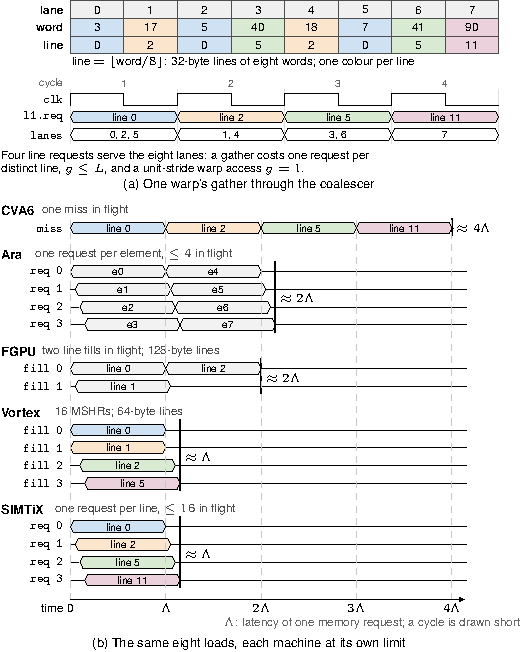
\includegraphics[width=\textwidth]{simtix_mem.pdf}
\caption{Memory-level parallelism. (a) A gather of one warp: the eight lane addresses
fall in four 32-byte lines, and the coalescer sends one line request per cycle for the
lowest pending lane together with the other lanes on its line. (b) The same eight
loads on CVA6, whose data cache has one miss-status register; on Ara, which sends one
request per element of a strided or indexed access with at most four in flight; and on
SIMTiX, which sends one request per line with up to 16 in flight while its other warps
keep issuing. $\Lambda$ is the memory latency.}
\label{fig:mem}
\end{figure*}

These structures set the memory-level parallelism of SIMTiX: up to 16 line requests,
from any warps, are in flight at once, limited by the 16 tags and the 16 MSHRs, and
meanwhile the scoreboard lets the warps whose operands are ready keep issuing.

\begin{proposition}\label{prop:mlp}
(a) A memory instruction whose $k$ active lanes access $g$ distinct lines costs $g$
line requests, $1\le g\le k$; a unit-stride access of $k\le L$ 32-bit words from a
line-aligned base has $g=1$. (b) If each lane draws its line independently and
uniformly from $R$ lines,
\begin{equation}
\mathbb{E}[g]=R\Bigl(1-\bigl(1-\tfrac{1}{R}\bigr)^{k}\Bigr).
\label{eq:eg}
\end{equation}
(c) A memory system that holds at most $M$ requests in flight, each of which takes at
least $\Lambda$ cycles, completes at most $M/\Lambda$ requests per cycle in the long
run.
\end{proposition}
\begin{IEEEproof}
(a) The coalescer sends one request per cycle for the lowest pending lane and removes
every pending lane on the same line, so each distinct line costs exactly one request.
A line holds $L$ words, so $k\le L$ consecutive words from a line-aligned base lie in
one line. (b) A given line is missed by all $k$ lanes with probability
$(1-1/R)^k$; summing the probability that each of the $R$ lines is touched gives
(\ref{eq:eg}) by linearity of expectation. (c) Each of the $M$ places in flight holds
one request for at least $\Lambda$ cycles, so over $T$ cycles it completes at most
$T/\Lambda+1$ requests (Little's law).
\end{IEEEproof}

By (\ref{eq:eg}), a gather into a small table coalesces and one into a large table
does not: the 16 bins of the histogram of Section~\ref{sec:evalamo} occupy $R=2$
lines, so eight lanes touch $\mathbb{E}[g]=1.99$ lines, while a gather into
$R=65{,}536$ lines touches 7.9996. For gathers of the second kind each request brings
one useful word, and part (c) bounds the useful words per cycle by $16/\Lambda$ for
SIMTiX, against $4/\Lambda$ for Ara and $1/\Lambda$ for CVA6
(Fig.~\ref{fig:mem}(b), Section~\ref{sec:machines}).

%==============================================================================
\section{Line-Aggregated Atomic Memory Operations}\label{sec:amo}
%==============================================================================
With one read-modify-write per lane, an AMO whose $k$ active lanes fall in one
line costs $k$ reads and $k$ writes, and behind a write-through L1 every write
also travels to DDR4. We aggregate the lanes by line instead. Let $P$ be the
pending lanes of an AMO context, $a_i$ the address of lane $i$, and $\ell=\min P$
the lead lane. The engine forms the group
$G=\{i\in P:\mathrm{line}(a_i)=\mathrm{line}(a_\ell)\}$ and
\begin{enumerate}
\item reads the line once into a line buffer;
\item applies the lanes of $G$ to the buffer in \emph{rounds}: a round applies
every remaining lane $i\in G$ for which no lower remaining lane of $G$ addresses
the same word; an applied lane receives the old word as its result and the buffer
word is replaced by the AMO's new value;
\item writes the line back with one request whose byte enables cover the words
that changed; and
\item removes $G$ from $P$ and repeats while $P$ is not empty.
\end{enumerate}
An RV32A AMO with operand $v_i$ replaces the word $x$ at $a_i$ by $f(x,v_i)$, where
$f$ is the AMO's operation (add, swap, and, or, xor, minimum or maximum), and returns
$x$ to lane $i$. Its \emph{serial} execution applies the active lanes one at a time
in ascending lane order.

\begin{theorem}\label{thm:amo}
Line-aggregated execution leaves memory as serial execution does and returns to every
lane the value that serial execution returns.
\end{theorem}
\begin{IEEEproof}
Fix a group $G$ and a word $w$ of its line, and let $i_1<i_2<\dots<i_m$ be the lanes
of $G$ on $w$. A round applies, for each word, only the lowest remaining lane on that
word, so the lanes applied in one round address different words and their updates
of the buffer are independent; and $w$ receives one lane per round in the order
$i_1,\dots,i_m$. The values returned to $i_1,\dots,i_m$ and the final value of $w$
depend only on the initial value of $w$ and this order, since $f$ reads and writes
only the addressed word. Serial execution applies the same lanes to $w$ in the same
order, starting from the same value, and so returns the same values and leaves the
same word. This holds for every word of the line. The line is read once before the
group and written back once after it, and the context holds the request port from
the read to the write, so no other request reaches the line in between; by
Theorem~\ref{thm:order} the read includes every earlier write. Different groups
cover disjoint sets of lines, so their order does not change the result.
\end{IEEEproof}

\begin{corollary}\label{cor:amo}
An AMO whose $k$ active lanes fall in $g$ lines costs $2g$ memory requests instead of
$2k$. A group $G$ takes $|G|$ apply cycles in the serial variant and
$m_G=\max_w|\{i\in G:\mathrm{word}(a_i)=w\}|$ in the parallel variant, the largest
number of its lanes on one word.
\end{corollary}
\begin{IEEEproof}
Each group costs one read and one write, and there are $g$ groups. The serial variant
applies one lane per cycle; in the parallel variant each round removes the lowest
remaining lane of every word, so the word with $m_G$ lanes takes $m_G$ rounds and
every other word is finished by then.
\end{IEEEproof}

The aggregation therefore needs no change to the kernel and no assumption that the
operation commutes: swap, minimum and maximum keep their serial results.
\begin{figure*}[t]
\centering
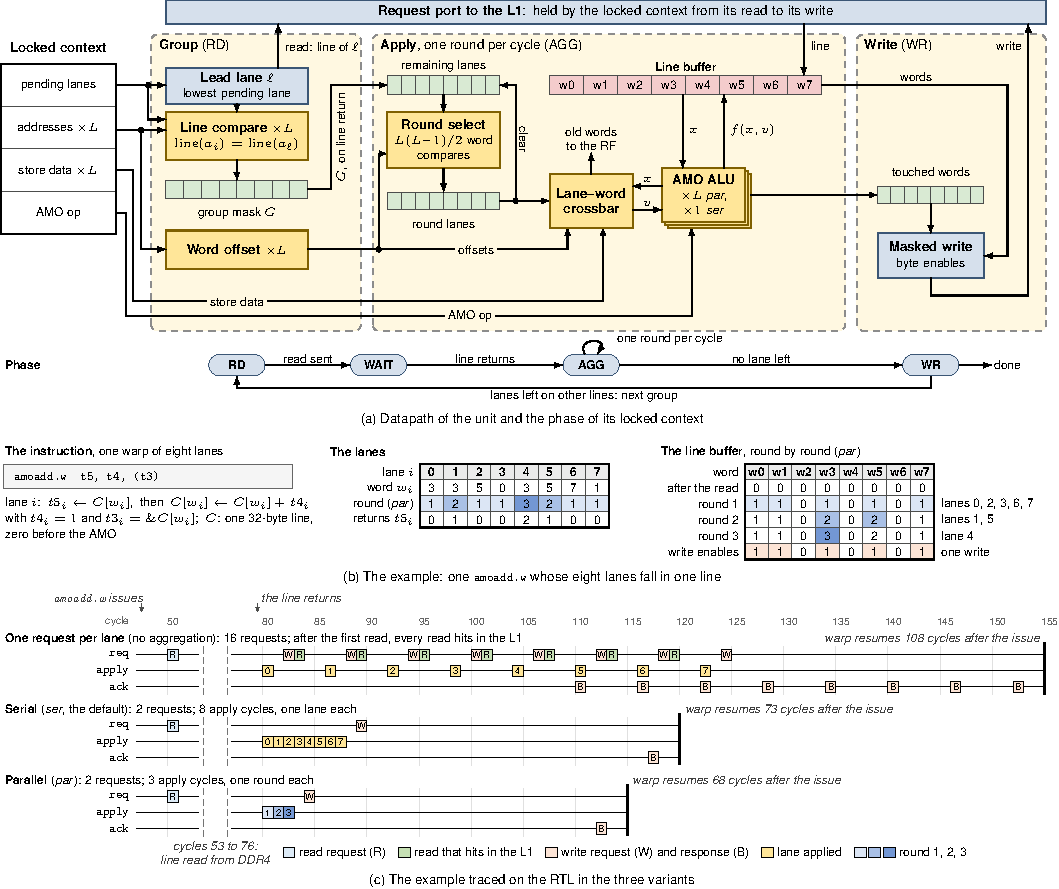
\includegraphics[width=\textwidth]{simtix_amo.pdf}
\caption{Line-aggregated AMOs. (a) Datapath of the unit in the parallel variant;
the serial variant applies the lowest remaining lane with one ALU and needs no word
compares. RD, WAIT, AGG and WR are the read, wait, apply and write states of the
context. (b) An AMO whose eight lanes address words of one line: lanes 0, 1 and 4
share word~3 and lanes 2 and 5 share word~5, so the parallel variant applies the
group in three rounds.}
\label{fig:amo}
\end{figure*}

Fig.~\ref{fig:amo}(a) shows the datapath. The lead lane and $L$ line
comparators form $G$, and the read request carries the line of $\ell$. When the
line returns, it is loaded into the line buffer and $G$ into the remaining-lanes
mask. In each cycle of the apply phase the round select picks the lanes of the
round, which takes $L(L{-}1)/2$ compares of word offsets, 28 at eight lanes. The
word multiplexers give each applied lane its old word, which returns to the RF
through the write arbiter in a cycle without a load write-back. The AMO ALUs
compute the new words, which replace their words in the buffer, and the words
written collect into the byte enables of the one masked write. A four-state
machine holds the request port from the read to the write.
Fig.~\ref{fig:amo}(b) follows one AMO instruction: per lane it needs 16 requests,
and aggregated it needs two, with eight apply cycles in the serial variant and
three in the parallel one.

We implemented both datapaths. The serial variant (\emph{ser}) has one AMO
arithmetic unit and applies the lowest remaining lane in each cycle, so the lanes
follow lane order; the parallel variant (\emph{par}) has one unit per word and
applies a whole round per cycle. Both return the same values. Each variant is a
build parameter, and we built the board design with each. The design without
aggregation uses 106,998 LUTs and the serial variant 107,658, 660 more (0.6\%);
both close timing at 115.4~MHz. The parallel variant uses 114,446 LUTs, 6,788
more than the serial one (6.3\%), and closes at 118.7~MHz. Out of context, where synthesis cannot share logic with the rest of
the design, the memory engine of the earlier four-warp design grew by 2,551 LUTs
(serial) and 5,923 (parallel). The serial variant is the default.

A dedicated kernel issues colliding \texttt{amoadd}, \texttt{amomax} and
\texttt{amoswap} instructions and checks every returned value and the final memory
against a serial model. It and a histogram run with and without aggregation under
seven memory configurations, from a zero-latency memory to the L1 with only two
sets, which forces evictions, and the L1 behind the AXI4 master with an
out-of-order memory model. On the board, the contention kernel runs with 262,144
threads under each variant, and the host checks all 786,432 returned values and
the 524,288 final words against the lanes executed one at a time in lane order.

%==============================================================================
\section{Implementation and Timing Closure}\label{sec:impl}
%==============================================================================
SIMTiX is written in SystemVerilog. Twenty-one self-checking testbenches, in 38
configurations of memory latency, ordering and cache, run under Vivado's simulator
and under Verilator~5.020 in continuous integration; before a bitstream is built,
the configuration it uses also runs at the board's input sizes, with write
responses delayed behind later reads. We implemented the designs with
Vivado~2025.1 for the XCZU9EG-2 device of the ZCU102 (274,080 LUTs, 548,160
flip-flops, 912 block RAMs and 2,520 DSP blocks). The board design is a block
design of the PS, an AXI SmartConnect and the accelerator, implemented in context
into the bitstream that runs on the board. Its clock comes from the PS, which
divides a 1.5~GHz phase-locked loop by an integer; we use 1.5~GHz$/13 =
115.37$~MHz. Every frequency we report is that of a routed design: with worst
setup slack WNS at the clock period $T$, \Fmax${}=1/(T-\mathrm{WNS})$. None is a
median over placement runs or an estimate before routing.

\subsection{Floating-Point Datapath}
The floating-point datapath is 2.5 times the area of the integer engine and,
placed, is limited by routing rather than by logic depth. With a two-stage FMA the
eight-lane engine closed at 78~MHz out of context, with its worst path in the
first FMA stage and 58\% of the delay in routing. Sharing one divide and
square-root unit among the lanes removed 3.7k LUTs and raised this to 84~MHz with
the FMA unchanged. A four-lane build reached only 79.7~MHz, which showed that the
limit lay inside one lane's FMA rather than in the total area. A three-stage FMA
then closed at 100.7~MHz and moved the worst path to the register-file read. In
the deployed unit the significand product is fully pipelined on DSP blocks, which
makes the unit five stages deep.

\subsection{Memory Path}\label{sec:closure}
Adding the L1 and the aggregated AMOs to the board design first missed 100~MHz by
2.478~ns with 16,301 failing endpoints. The worst path was a single-cycle loop of
30 logic levels, 76\% of it routing: from the pending-lane masks of a memory
context through port arbitration and address selection into the L1 tag compare,
the hit, the completion of the context and the warp's resume into the PC of its
reconvergence stack. Four changes closed it. The L1 registers its input. A
context completes from registered state and the cycle's responses, which is valid
for a memory that never answers in the request cycle. The L1 chooses one cycle
ahead which waiting read it answers next. A post-route physical optimization pass
was added. The input register costs 1.5--2.5\% of the total cycles of the
applications.

\subsection{Issue Logic and Memory Engine Beyond 100~MHz}\label{sec:clock}
With the register scoreboard and the result queues, the board design first closed
at 100~MHz with little margin ($+0.093$~ns at four warps, $+0.261$~ns at eight).
In the routed four-warp design, 38,680 timing endpoints fail at 150~MHz, 12,087 at 125~MHz and about 2,455 at 111~MHz, in four
groups: warp issue into the memory engine's context registers, warp issue into
the reconvergence stack, the memory engine's request choice into the L1 input
register, and the first and last stages of the lane FPUs. Reaching 150~MHz would
need an operand-read stage across the whole issue logic, so we cut the four
groups instead. The memory engine registers its input, its chosen request (the
choice among the contexts in one cycle, the line address and data in the next)
and the resumption of a warp; a branch or jump updates the reconvergence stack in
stage B; and synthesis retiming balances the FPU stages. Together these add
0.3--3.8\% to the cycles of the applications, and the board design closes at
115.37~MHz with $+0.406$~ns of slack, an \Fmax\ of 121.0~MHz. Its worst path is
now inside a lane FPU (34 logic levels, 70\% of the delay in routing).

\begin{table}[t]
\caption{Board Designs on the XCZU9EG-2 at 115.37~MHz}
\label{tab:impl}
\centering\footnotesize
\setlength{\tabcolsep}{2.4pt}
\begin{tabular}{lrrrrrr}
\toprule
Design & LUT & FF & BRAM & DSP & \Fmax & Power$^a$\\
 & & & & & (MHz) & (W)\\
\midrule
8 lanes, \emph{ser} AMOs   & 107,658 & 50,091 & 16 & 72 & 121.0 & 1.08\\
8 lanes, no aggregation    & 106,998 & 50,036 & 16 & 72 & 120.2 & 1.16\\
8 lanes, \emph{par} AMOs   & 114,446 & 50,053 & 16 & 72 & 118.7 & 1.35\\
\bottomrule
\end{tabular}

\vspace{2pt}
\begin{minipage}{\columnwidth}\footnotesize
Each row is a complete board design (PS, interconnect, accelerator), implemented
in context; resources are the whole design's, almost all of them the
accelerator's. BRAM counts RAMB36 tiles. $^a$Vivado's estimate for the
accelerator; the PS adds 2.74~W. Measured power: Section~\ref{sec:evalboard}.
\end{minipage}
\end{table}

Table~\ref{tab:impl} lists the board designs. The default design uses 39\% of the
device's LUTs and 9\% of its flip-flops. Of its 16 block RAMs, all hold the L1's
data; the register files, the L1 tags and the scratchpad are in LUTRAM.

%==============================================================================
\section{Evaluation}\label{sec:eval}
%==============================================================================
\subsection{Four Machines on One Board}\label{sec:machines}
\begin{table}[t]
\caption{The Four Machines on the ZCU102}
\label{tab:machines}
\centering\footnotesize
\setlength{\tabcolsep}{3.0pt}
\begin{tabular}{lllll}
\toprule
 & SIMTiX & Vortex & Ara & CVA6\\
\midrule
Type & SIMT $8\times8$ & SIMT $8\times8$ & vector & scalar\\
ISA & RV32IAF$^a$ & RV32IMAF & RVV 1.0 & RV64GC\\
Clock (MHz) & 115.37 & 125 & 78.95 & 78.95\\
Peak $P$ (op/cycle) & 8 & 8 & 4 & 1\\
FP32 GFLOP/s & 1.85 & 2.00 & 0.63 & 0.16\\
Divergence & stack & split/join & masks & branch\\
L1 D (KB, line) & 64, 32~B & 16, 64~B & none & 8, 32~B\\
In flight & 16 lines & 16 MSHRs & 4 elem.$^b$ & 1 miss\\
Divide, sqrt & 1 shared & per lane & per lane & 1\\
\midrule
LUT & 107,658 & 85,179 & \multicolumn{2}{c}{182,331}\\
FF & 50,091 & 85,577 & \multicolumn{2}{c}{63,650}\\
BRAM / DSP & 16 / 72 & 62 / 48 & \multicolumn{2}{c}{92.5 / 130}\\
\bottomrule
\end{tabular}

\vspace{2pt}
\begin{minipage}{\columnwidth}\footnotesize
$8\times8$: eight warps of eight threads; Ara has two lanes. Peak $P$: 32-bit operations started per cycle,
an FMA counted as one; GFLOP/s count an FMA as two. L1: SIMTiX and CVA6 write through,
Vortex writes back, all four-way. Resources: the whole board design; Ara and CVA6 are
one design. In flight: memory requests. $^a$With Zfh, Zba, Zbb, Zicond and \texttt{mul} of M. $^b$Elements of a
strided or indexed access; unit-stride accesses become AXI4 bursts.
\end{minipage}
\end{table}

We compare SIMTiX with three RISC-V machines of different organization
(Table~\ref{tab:machines}). Each is a separate bitstream for the same ZCU102, built with
the same Vivado flow and driven by the same A53 host program. CVA6~\cite{cva6} is a
single-issue, in-order 64-bit core, the kind of scalar processor that an accelerator in
the logic must outperform. Ara~\cite{ara,ara2} is a vector processor of the RISC-V
vector extension (RVV~1.0), whose instructions CVA6 issues; with two lanes it has
2,048-bit vector registers. CVA6 also runs the scalar code of every benchmark without
the vector unit, and the two form one design, which closes at 78.95~MHz.
Vortex~\cite{vortex} is a SIMT GPGPU; we built one core with the warp count and width
of SIMTiX, eight warps of eight threads, which closes at 125~MHz.

The peak $P$ of a machine is the number of 32-bit operations it can start per cycle,
counting an FMA as one. It is eight for SIMTiX and Vortex, which issue one warp
instruction of eight lanes per cycle; four for Ara, whose two lanes each operate on
two FP32 or INT32 elements of a 64-bit datapath; and one for CVA6. The memory systems
differ more than the peaks. CVA6's write-through data cache has one miss-status
register, so one miss is in flight. Ara's load-store unit turns a unit-stride access
into AXI4 bursts but sends one single-beat request per element of a strided or indexed
access, with at most four in flight. SIMTiX sends one request per line touched, with
up to 16 in flight (Section~\ref{sec:l1}).

\subsection{Rodinia on Four Machines}\label{sec:rodinia}
\begin{table*}[t]
\caption{Applications and Rodinia on the ZCU102: Time of SIMTiX, CVA6, Ara, Vortex and
the A53, and Each Time Divided by SIMTiX's}
\label{tab:rodinia}
\centering\footnotesize
\setlength{\tabcolsep}{3.2pt}
\begin{tabular}{llrrrrrrrrr}
\toprule
Benchmark & Input & SIMTiX & \multicolumn{2}{c}{CVA6} & \multicolumn{2}{c}{Ara}
 & \multicolumn{2}{c}{Vortex} & \multicolumn{2}{c}{A53}\\
\cmidrule(lr){4-5}\cmidrule(lr){6-7}\cmidrule(lr){8-9}\cmidrule(lr){10-11}
 & & (ms) & (ms) & ratio & (ms) & ratio & (ms) & ratio & (ms) & ratio\\
\midrule
\multicolumn{11}{l}{\emph{Applications of Table~\ref{tab:board}}}\\
GEMM-RB    & $256^3$                       & 37.8    & 3,689.7   & 97.7 & 77.4     & 2.05 & 198.2    & 5.25 & 169.6    & 4.49\\
SpMV-Z     & 65,536 rows                   & 19.3    & 362.3     & 18.7 & 313.2    & 16.2 & 46.2     & 2.39 & 18.3     & 0.95\\
CNN        & $128^2$, 16-32-32 channels    & 290.7   & 27,266.5  & 93.8 & 1,581.3  & 5.44 & 2,066.4  & 7.11 & 1,191.9  & 4.10\\
Mandelbrot & $1024^2$, 256 iterations      & 1,019.7 & 11,142.5  & 10.9 & 4,553.5  & 4.47 & 5,324.0  & 5.22 & 846.8    & 0.83\\
\midrule
\multicolumn{11}{l}{\emph{Rodinia}}\\
pathfinder & 100 rows, 100,000 columns   & 250.5   & 4,428.8   & 17.7 & 421.2    & 1.68 & 960.9    & 3.84 & 97.2     & 0.39\\
backprop   & 2$^{19}$ inputs, 16 hidden    & 299.2   & 5,729.0   & 19.1 & 3,055.4  & 10.2 & 1,008.8  & 3.37 & 214.2    & 0.72\\
bfs        & graph65536                    & 36.7    & 299.8     & 8.17 & 794.1    & 21.7 & 126.8    & 3.46 & 21.9     & 0.60\\
hotspot    & $512^2$, 2 iterations         & 33.6    & 553.1     & 16.5 & 45.3     & 1.35 & 103.0    & 3.07 & 21.0     & 0.63\\
hotspot    & $1024^2$, 2 iterations        & 134.2   & 2,475.0   & 18.4 & 172.8    & 1.29 & 411.2    & 3.06 & 85.5     & 0.64\\
nn         & 42,764 records                & 15.3    & 24.4      & 1.59 & 8.9      & 0.58 & 4.8      & 0.31 & 1.0      & 0.07\\
hotspot3D  & $512^2\times8$, 100 iterations & 9,449.6 & 491,642.8 & 52.0 & 20,528.6 & 2.17 & 21,504.5 & 2.28 & 16,522.7 & 1.75\\
gaussian   & $1024\times1024$              & 4,965.0 & 104,642.3 & 21.1 & 10,176.9 & 2.05 & 6,064.0  & 1.22 & 3,916.4  & 0.79\\
kmeans     & kdd\_cup, $k=5$, 37 iterations & 31,810.0 & 726,014.0 & 22.8 & 56,290.0 & 1.77 & 64,442.3 & 2.03 & 28,064.9 & 0.88\\
\midrule
\multicolumn{3}{l}{Geometric mean of the ratio, Rodinia, time} & & 14.6 & & 2.62 & & 1.98 & & 0.56\\
\multicolumn{3}{l}{Geometric mean of the ratio, Rodinia, clock cycles} & & 9.97 & & 1.79 & & 2.15 & & ---\\
\multicolumn{3}{l}{Geometric mean of the ratio, all twelve, time} & & 19.9 & & 3.32 & & 2.63 & & 0.85\\
\multicolumn{3}{l}{Geometric mean of the ratio, all twelve, clock cycles} & & 13.6 & & 2.27 & & 2.85 & & ---\\
\bottomrule
\end{tabular}

\vspace{2pt}
\begin{minipage}{\textwidth}\footnotesize
Clocks: SIMTiX 115.4~MHz, CVA6 and Ara 78.95~MHz, Vortex 125~MHz, A53 1.2~GHz. Ratio:
the machine's time (or cycles) divided by SIMTiX's; above 1 favors SIMTiX. Geometric
means with hotspot at $1024^2$. SIMTiX runs the GEMM-RB and SpMV-Z kernels of
Table~\ref{tab:board}; Vortex runs SIMTiX's base GEMM and SpMV kernels, ported. A53:
the \texttt{-O2} reference (Table~\ref{tab:board} gives the faster of \texttt{-O2} and
\texttt{-O3}). Every output is checked against the A53 reference: exact for SIMTiX and
Vortex; for CVA6 and Ara exact except nn (at most 1~ulp) and gaussian (at most
$2.2\times10^{-4}$ of each row's largest value; limit $10^{-3}$).
\end{minipage}
\end{table*}

We ran four applications of Table~\ref{tab:board} (GEMM, SpMV, the CNN and
Mandelbrot) and eight benchmarks of the Rodinia suite~\cite{rodinia} on the four
machines. In every run the A53 loads the program, loads or generates the inputs,
computes the reference results and checks every output.

The four applications use the inputs and the A53 references of
Table~\ref{tab:board}. Each Rodinia benchmark is defined by Rodinia's computation on
Rodinia's data: the sequence of
FP32 operations that produces one output, each rounded once, with a fused multiply-add
where the sum is fused. Every machine performs these operations in this order, in its
own parallel form: one output per thread on SIMTiX and Vortex, per vector element on
Ara and per loop iteration on CVA6 and the A53. The SIMTiX kernels are hand-written
assembly. Vortex runs C++ versions of the same algorithms compiled by its LLVM
toolchain; Ara runs C with vector intrinsics; CVA6 and the A53 run one C reference,
compiled with GCC. The input files are Rodinia's own. Work that Rodinia performs on the
CPU (the control of the bfs levels, the selection of the nearest records in nn, the
centre update of kmeans and the back substitution of gaussian) runs on the A53 for
every machine and is not timed. For SIMTiX and Vortex, the A53's timer measures from the
first launch to the end of the last, including the host's work between launches; for
CVA6 and Ara, the cycle counter of CVA6 measures the kernel, whose loop over iterations
runs on CVA6 itself.

Three choices depart from Rodinia's default runs. All machines compute in FP32.
backprop uses 2$^{19}$ inputs rather than 2$^{21}$, whose two 256~MB weight arrays do
not fit the memory region of the Ara host. gaussian uses the matrix that Rodinia
generates rather than its matrix file: Rodinia eliminates without pivoting, and on the
random matrix of the file the entries grow to $5.3\times10^{4}$, so that a change of
one ulp in 8.7\% of the quotients changes rows of the result by up to 6.3 times their
largest entry. This matters because the divide and square-root unit of CVA6, which Ara
shares, is not correctly rounded: on 4,096 random operands, 8.7\% of its quotients and
6.9\% of its square roots differ from the correctly rounded value by one ulp. CVA6 and
Ara are therefore checked within a tolerance in the two benchmarks that divide or take
a square root, and exactly in the others. Finally, Ara computes gaussian's multipliers
(Rodinia's Fan1 kernel, one division per row) on CVA6, because its vector form returned
wrong values, or deadlocked, when it ran after nn; the elimination itself (Fan2) runs
on Ara.

\begin{figure*}[t]
\centering
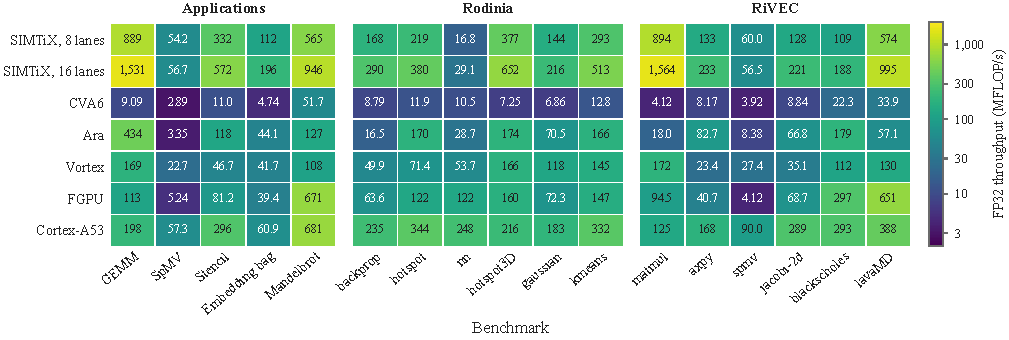
\includegraphics[width=\textwidth]{machines_heatmap.pdf}
\caption{Speed-up of SIMTiX over CVA6, Ara and Vortex on the ZCU102 for the
applications, Rodinia and RiVEC: the time of a machine divided by the time of the
eight-lane SIMTiX (left three columns of each panel) and of the 16-lane SIMTiX of
Section~\ref{sec:lanes16} (right three columns). Blue: SIMTiX is faster; red: the other
machine is (logarithmic color scale, saturated beyond $32\times$). Each benchmark at its
largest input (Rodinia's hotspot at $1024^2$); all times measured; boxed rows: geometric
means over the benchmarks of the suite. n/a: wrong outputs (Ara's MLP and
Smith-Waterman) or a deadlock (Ara's Mandelbrot).}
\label{fig:mach_heatmap}
\end{figure*}

Fig.~\ref{fig:mach_heatmap} compares the four machines on the twelve applications of
Table~\ref{tab:board}, Rodinia and RiVEC (Section~\ref{sec:rivec}). For each benchmark
at its largest input, a cell gives the time of a machine divided by SIMTiX's, for the
eight-lane SIMTiX and for the 16-lane SIMTiX of Section~\ref{sec:lanes16}. Over these
inputs, the eight-lane SIMTiX is $21.2\times$, $6.0\times$ and $4.1\times$ faster than
CVA6, Ara and Vortex on the applications (geometric means; Table~\ref{tab:rodinia}
averages both input sizes); the 16-lane SIMTiX raises these to $32.9\times$,
$8.9\times$ and $6.4\times$. Another machine is faster only where the work is division
and square root: Ara on RiVEC's Black-Scholes, Vortex by 2.5\% on the same kernel, and
Ara and Vortex on nn (below). Ara's MLP and Smith-Waterman outputs are wrong on the
board and Mandelbrot deadlocks Ara, so these three are not compared.

Sections~\ref{sec:evallanes} and~\ref{sec:lanes16} also use a second suite of ten kernels,
\emph{suite~2}, drawn from five benchmark suites: pathfinder, hotspot and backprop from
Rodinia, Black-Scholes from RiVEC, PageRank and connected components from
GAP~\cite{gap}, the radix sort of SHOC~\cite{shoc}, and ATAX, BiCG and Jacobi-2D from
PolyBench~\cite{polybench}. Suite~2 follows the rules of the applications: each kernel
is defined by the sequence of FP32 operations of one output, SIMTiX runs hand-written
assembly, the A53 runs one C version and checks every output, and every kernel runs at
two input sizes.

Table~\ref{tab:rodinia} and Fig.~\ref{fig:mach_heatmap} give the results, and
Fig.~\ref{fig:decomp}(b) the efficiency factor of each Rodinia benchmark. On the four applications SIMTiX is faster than every other
machine: by 10.9 to $97.7\times$ than CVA6, 2.05 to $16.2\times$ than Ara and 2.39 to
$7.11\times$ than Vortex. Over all twelve benchmarks the geometric means of the time
ratio are $19.9\times$ for CVA6, $3.32\times$ for Ara and $2.63\times$ for Vortex.
On Rodinia, SIMTiX is faster than CVA6 on every
benchmark, by $14.6\times$ in time on the geometric mean and $10.0\times$ per cycle. It
is $2.62\times$ faster than Ara in time and $1.79\times$ per cycle; the largest
margins are on bfs ($21.7\times$) and backprop ($10.2\times$). On the hotspot stencil,
whose rows Ara loads with unit stride, Ara comes within $1.3\times$ of SIMTiX in time
and needs 8 to 12\% fewer cycles. Against Vortex, which runs the same algorithms,
SIMTiX is $1.98\times$ faster in time and $2.15\times$ per cycle, from $1.22\times$ on
gaussian to $3.84\times$ on pathfinder.

nn is the one benchmark on which SIMTiX is slower than Ara and Vortex. It computes one
square root per record and little else. SIMTiX computes square roots in its single
shared divide unit, through which the active lanes pass in turn
(Section~\ref{sec:arch}), and needs 41 cycles per record; Vortex has one square-root
unit per lane, and Ara applies its square-root instruction to whole vectors. The A53,
at 10.4 times SIMTiX's clock, is faster than SIMTiX on seven of the eight benchmarks;
SIMTiX is faster on hotspot3D ($1.75\times$), whose two 8~MB grids are read and
written in every iteration.

\subsection{RiVEC on Four Machines}\label{sec:rivec}
\begin{table*}[t]
\caption{RiVEC on the ZCU102: Time of SIMTiX, CVA6, Ara, Vortex and the A53, and Each
Time Divided by SIMTiX's}
\label{tab:rivec}
\centering\footnotesize
\setlength{\tabcolsep}{3.2pt}
\begin{tabular}{llrrrrrrrrr}
\toprule
Application & Input & SIMTiX & \multicolumn{2}{c}{CVA6} & \multicolumn{2}{c}{Ara}
 & \multicolumn{2}{c}{Vortex} & \multicolumn{2}{c}{A53}\\
\cmidrule(lr){4-5}\cmidrule(lr){6-7}\cmidrule(lr){8-9}\cmidrule(lr){10-11}
 & & (ms) & (ms) & ratio & (ms) & ratio & (ms) & ratio & (ms) & ratio\\
\midrule
axpy         & 2,097,152 elements             & 31.5 & 513.4 & 16.3 & 50.7 & 1.61 & 179.2 & 5.69 & 25.0 & 0.80 \\
matmul       & $512^3$, RiVEC data            & 300.3 & 65,174.2 & 217 & 14,918.2 & 49.7 & 1,562.4 & 5.20 & 2,152.8 & 7.17 \\
spmv         & poisson3Db, $A^{\mathsf T}x$   & 79.2 & 1,211.9 & 15.3 & 567.1 & 7.16 & 173.6 & 2.19 & 52.8 & 0.67 \\
jacobi-2d    & $256^2$, 2,000 steps           & 10,116.6 & 145,978.7 & 14.4 & 19,324.5 & 1.91 & 36,713.8 & 3.63 & 4,461.7 & 0.44 \\
pathfinder   & $1024\times2048$, 100 runs     & 5,556.7 & 116,179.1 & 20.9 & 8,907.6 & 1.60 & 22,044.9 & 3.97 & 2,473.0 & 0.45 \\
blackscholes & 65,536 options, 100 runs       & 9,328.3 & 45,462.0 & 4.87 & 5,665.7 & 0.61 & 9,095.9 & 0.98 & 3,460.8 & 0.37 \\
lavaMD       & $10^3$ boxes of 96 particles   & 15,868.0 & 268,712.8 & 16.9 & 159,494.0 & 10.1 & 69,823.7 & 4.40 & 23,438.5 & 1.48 \\
\midrule
\multicolumn{3}{l}{Geometric mean of the ratio, time} & & 20.1 & & 3.76 & & 3.27 & & 0.88\\
\multicolumn{3}{l}{Geometric mean of the ratio, clock cycles} & & 13.8 & & 2.59 & & 3.53 & & ---\\
\bottomrule
\end{tabular}

\vspace{2pt}
\begin{minipage}{\textwidth}\footnotesize
Clocks and ratio as in Table~\ref{tab:rodinia}. Ara runs RiVEC's own vector code; SIMTiX
runs its GEMM-RB and SpMV-Z kernels for matmul and spmv, and Vortex its base GEMM and
SpMV kernels. All machines compute in FP32. Every output is checked against the A53
reference: exact for SIMTiX, Vortex and CVA6, and for Ara except in spmv and lavaMD
(at most $3.7\times10^{-6}$ of the sum of the magnitudes of the terms); blackscholes on
CVA6 and Ara at most $5.7\times10^{-4}$ of $|p|+0.01$ for a price $p$ (limit
$10^{-3}$).
\end{minipage}
\end{table*}

RiVEC~\cite{rivec} is a suite of applications vectorized for the RISC-V vector
extension by its authors. We ran seven of them on the four machines of
Section~\ref{sec:rodinia}: axpy, matmul and spmv from dense and sparse linear algebra,
the jacobi-2d stencil of PolyBench, pathfinder and lavaMD from Rodinia, and the
blackscholes option pricing of PARSEC, with RiVEC's largest inputs. On Ara each
application runs RiVEC's own vector code, written with RVV~1.0 intrinsics; this tests
Ara with code that its instruction set was designed for, written by others. The other
machines run the computation of RiVEC's code in the forms of
Section~\ref{sec:rodinia}: hand-written assembly on SIMTiX, C++ compiled by LLVM on
Vortex, and one C reference compiled by GCC on CVA6 and the A53. RiVEC computes in
FP64; all machines here compute in FP32, the precision of SIMTiX and Vortex.

Each application is defined by RiVEC's vector code read per element: the FP32
operations that produce one output element, with RiVEC's fused multiply-adds and its
polynomial exponential and logarithm. Sums over many elements (a row of spmv, the
force on a particle in lavaMD) are defined in serial order. SIMTiX, Vortex and CVA6
then produce the A53 reference bit for bit, and so does Ara except in spmv and lavaMD,
where its code keeps one partial sum per vector element and reduces them at the end.
blackscholes divides three times and takes one square root per option; with the divide
and square-root unit of CVA6 (Section~\ref{sec:rodinia}), CVA6 and Ara give identical
prices that differ from the reference by up to $5.7\times10^{-4}$ of $|p|+0.01$. A
model of RiVEC's computation in which each quotient and square root is one ulp off at
the measured rates of 8.7\% and 6.9\% gives the same bound,
$5.7\times10^{-4}$, over 200 random trials on the same options; the limit is
$10^{-3}$.

RiVEC's code was changed in four places. Two are errors in RiVEC. Its blackscholes
negates the cumulative normal of the negative arguments with a masked subtract in the
mask-agnostic form, which allows an RVV~1.0 implementation to overwrite the
unselected elements; under QEMU, 46,277 of the 65,536 prices are wrong. We select the
two results with a merge instead. RiVEC's spmv builds the matrix from the file's
column-major entries with one-based indices and reads one element past the end of $x$;
we use zero-based indices, which computes $y=A^{\mathsf T}x$ for RiVEC's matrix. The
other two changes avoid faults of Ara. Ara reloads a vector register spilled to the
stack with wrong values, and GCC spills one in blackscholes, so RiVEC's code is
compiled with clang, which does not. Ara's jacobi-2d computed wrong last elements of
some rows, differently from run to run, when it ran after another kernel, while it
reused vector registers from one row to the next; it now loads the three rows for
every output row, which costs about 46\% more cycles in a reduced run.

Table~\ref{tab:rivec} and Fig.~\ref{fig:mach_heatmap} give the results.
SIMTiX is faster than CVA6 on every application, by $20.1\times$ in time on the
geometric mean and $13.8\times$ per cycle, and faster than Vortex on six of the
seven, by $3.27\times$ in time and $3.53\times$ per cycle. Against Ara the geometric
mean is $3.76\times$ in time and $2.59\times$ per cycle, with a wide spread. RiVEC's
matmul forms each element of the product as a dot product whose loads run down a
column of $B$ with a stride of one row, and Ara takes $49.7\times$ SIMTiX's time; on
lavaMD and spmv, which reduce per particle and per row, the ratios are $10.1$ and
$7.16\times$. On the three applications that stream rows with unit stride (axpy,
pathfinder and jacobi-2d) SIMTiX is 1.60 to $1.91\times$ faster in time and Ara needs
only 10 to 31\% more cycles.

blackscholes is the one application on which SIMTiX is not the fastest accelerator:
Ara takes 0.61 of its time and 0.42 of its cycles, and Vortex is level
($0.98\times$). As in nn (Section~\ref{sec:rodinia}), the three divisions and the
square root of each option pass lane by lane through SIMTiX's single divide unit,
while Ara applies its divide and square-root instructions to whole vectors and Vortex
has a unit per lane. The A53 is faster than SIMTiX on five of the seven applications
($0.88\times$ on the geometric mean). SIMTiX is faster on lavaMD ($1.48\times$),
whose force computation has many operations per particle pair, and on matmul
($7.17\times$). There the A53 runs RiVEC's loop order, whose inner loop reads a column
of the 1~MB matrix $B$ with a stride of 2~KB; this stride maps the 512 elements of the
column onto 4 of the 128 sets of the A53's 32~KB four-way L1 data cache, which
therefore cannot hold one column.

\subsection{Where the Speed-Up Comes From}\label{sec:decomp}
\begin{figure*}[t]
\centering
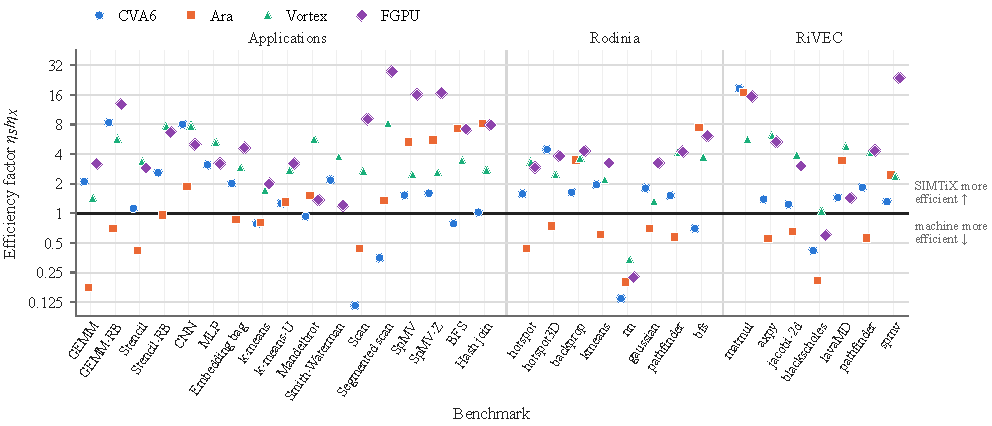
\includegraphics[width=\textwidth]{decomp.pdf}
\caption{The time ratio of each machine over SIMTiX split into its three factors by
(\ref{eq:decomp}), over the eight Rodinia benchmarks (hotspot at $1024^2$) and the
seven RiVEC applications. (a) Geometric means of the clock, peak and efficiency
factors and of their product, the time ratio. (b) The efficiency factor of each
benchmark, ordered by Ara's; above 1, SIMTiX sustains a larger fraction of its peak
than the other machine.}
\label{fig:decomp}
\end{figure*}

Let a benchmark take time $T_S$ and $C_S$ cycles on SIMTiX at clock frequency $f_S$,
and $T_X$ and $C_X$ cycles on machine $X$ at $f_X$. Let $N$ be the number of 32-bit
operations of its computation, which is the same on every machine, and
$\eta=N/(PC)$ the fraction of its peak that a machine sustains, its
\emph{efficiency}. Since $T=C/f$ and $C=N/(P\eta)$,
\begin{equation}
\frac{T_X}{T_S}=\frac{f_S}{f_X}\cdot\frac{P_S}{P_X}\cdot\frac{\eta_S}{\eta_X}.
\label{eq:decomp}
\end{equation}
The three factors are the clock, the width and how well each machine keeps its
datapath busy. $N$ cancels in the efficiency factor,
$\eta_S/\eta_X=(C_X/C_S)(P_X/P_S)$, which therefore follows from the measured cycles
and the peaks of Table~\ref{tab:machines} without counting operations. Instructions
that compute addresses, control loops or handle divergence lower $\eta$, as do cycles
in which the datapath waits.

Fig.~\ref{fig:decomp}(a) gives the geometric means over the 15 benchmarks of
Tables~\ref{tab:rodinia} and~\ref{tab:rivec}. Against CVA6, the time ratio of 16.95 is
1.46 from the clock, 8.00 from the width and 1.45 from efficiency. Against Ara, the
clock contributes 1.46 and the width 2.00, and the efficiency factor is 1.06: per
cycle, SIMTiX's lead over Ara is its width. Fig.~\ref{fig:decomp}(b) shows that this
mean hides two groups. On the ten benchmarks on the left, which stream rows with unit
stride or divide, Ara's efficiency is higher, by factors of 0.44 to 0.75 on the
streams: Ara turns their accesses into bursts and keeps more of its four operations
per cycle busy than SIMTiX of its eight. On the five on the right, which gather, read
with a stride or reduce per element, SIMTiX's efficiency is 2.4 (spmv) to 17.0
(matmul) times Ara's, as the limits on requests in flight of Section~\ref{sec:l1}
predict. Against Vortex, whose clock is 8\% higher and whose width is the same, the
whole factor of 2.71 is efficiency: Vortex executes more warp instructions for the
same computation and, with its longer pipeline, reaches a lower IPC at eight warps
(Section~\ref{sec:evalvortex}).

Outside Ara's streaming group, the efficiency factor is below 1 only on nn,
blackscholes and bfs. nn and blackscholes are bound by division and square root,
which SIMTiX passes lane by lane through one shared unit (Section~\ref{sec:arch}),
while Ara and Vortex have a unit per lane; bfs diverges, so many of SIMTiX's lanes
are idle while a warp follows its longest adjacency list, and CVA6, which processes
one vertex at a time, loses nothing to divergence. These are the two limits of the
present design that a later version can address: a pipelined divide through the FMA
units and a narrower issue for divergent code.

\subsection{Applications Against the Cortex-A53}\label{sec:evalboard}
\begin{table}[t]
\caption{Applications on the ZCU102: SIMTiX at 115.4~MHz Against One Cortex-A53
Core at 1.2~GHz}
\label{tab:board}
\centering\footnotesize
\setlength{\tabcolsep}{2.2pt}
\begin{tabular}{lrrrrrr}
\toprule
App. & \multicolumn{2}{c}{A53} & SIMTiX & Speed- & \multicolumn{1}{c}{Power (W)} & Energy\\
\cmidrule(lr){2-3}
 & (ms) & build & (ms) & up & A53 / SIMTiX & ratio\\
\midrule
Hash join       & 195.4   & O3 & 99.3    & 1.97 & 3.13 / 4.12 & 1.50\\
CNN             & 381.8   & O3 & 290.7   & 1.31 & 3.11 / 4.00 & 1.02\\
GEMM-RB         & 47.2    & O3 & 37.8    & 1.25 & 3.17 / 4.22 & 0.94\\
Embedding bag   & 45.4    & O3 & 37.5    & 1.21 & 3.12 / 4.05 & 0.94\\
BFS             & 194.6   & O3 & 162.9   & 1.19 & 3.13 / 3.88 & 0.96\\
SpMV-Z          & 18.1    & O3 & 19.4    & 0.94 & 3.17 / 4.08 & 0.73\\
Mandelbrot      & 845.7   & O3 & 1,019.7 & 0.83 & 3.12 / 4.19 & 0.62\\
Smith-Waterman  & 922.1   & O2 & 1,613.4 & 0.57 & 3.16 / 3.83 & 0.47\\
k-means-U       & 34.3    & O3 & 72.2    & 0.47 & 3.11 / 3.86 & 0.38\\
Stencil-RB      & 8.6     & O3 & 18.9    & 0.45 & 3.20 / 4.26 & 0.34\\
MLP             & 55.4    & O3 & 189.8   & 0.29 & --- & ---\\
Segmented scan  & 4.5     & O3 & 35.5    & 0.13 & 3.27 / 3.91 & 0.11\\
\bottomrule
\end{tabular}

\vspace{2pt}
\begin{minipage}{\columnwidth}\footnotesize
Large inputs: hash join 2$^{22}$ slots, 2$^{20}$ probes; CNN $128^2$, 16-32-32
channels; GEMM $256^3$; embedding bag 2$^{18}$ rows of 32 floats, 4,096 bags of 32;
BFS 2$^{18}$ vertices; SpMV 65,536 rows; Mandelbrot $1024^2$, 256 iterations;
Smith-Waterman 16,384 pairs of 32 and 128 bases; k-means 2$^{18}$ points, 16
clusters; stencil $512^2$, 4 sweeps; MLP 784-256-128-10, batch 256; scan 2$^{20}$.
A53: the faster of the \texttt{-O2} and \texttt{-O3 -mcpu=cortex-a53} builds.
Power: sum of the 18 monitored rails while the application runs. Energy ratio: A53
energy over SIMTiX energy, each run time times total power; above 1 favors SIMTiX.
\end{minipage}
\end{table}

The host program runs every application on its large input, first on the
accelerator and then on one A53 core with an ordinary sequential algorithm in C: a
queue for BFS, a running sum for the scan, the $i$-$k$-$j$ loop order for GEMM, and
for the CNN and the MLP the usual CPU layouts (channels and the dot products'
operands contiguous). We built the references with \texttt{-O2} and with
\texttt{-O3 -mcpu=cortex-a53}, with which GCC vectorizes with NEON, and report the
faster build. They are compiled C, not a hand-tuned library. The FP32 references
perform the kernels' operations in the same order, so every output of the
accelerator is compared exactly with the A53's; both builds produce the same
results. Times come from the A53's global timer; the accelerator time runs from
the first GO to the last DONE and includes the host's work between launches. For
power, each phase (idle, accelerator, A53) is repeated for 2~s, and between
repetitions, at most every 50~ms, the host reads the board's 18 INA226 monitors
over I$^2$C, ten on the processing system's rails and eight on the programmable
logic's.

Table~\ref{tab:board} gives the results. SIMTiX is faster than the A53 on five
applications. Three are limited by memory latency: the hash-join probe ($1.97\times$),
the embedding bag ($1.21\times$) and BFS ($1.19\times$) gather from random lines of
tables far larger than the A53's 1~MB L2 cache, and the in-order A53 waits on each
miss, while SIMTiX keeps 64 threads and 16 misses in flight. The other two, the CNN
($1.31\times$) and the register-blocked GEMM ($1.25\times$), reuse each loaded
operand several times per thread. SIMTiX is slower on kernels with little work per
element (the scan, the stencil, k-means), on scalar dynamic programming
(Smith-Waterman, $0.57\times$), on Mandelbrot ($0.83\times$), and on the MLP, whose
contiguous INT8 dot products the A53 vectorizes. With one output per thread, the
MLP kernel issues 0.32~G multiply-adds per second, against 0.78~G for the CNN
kernel, which computes four.

The energy is less favorable. With every rail counted, the board draws
3.13--3.17~W idle with the A53 polling the accelerator, 3.11--3.27~W while the A53
computes and 3.62--4.26~W while SIMTiX runs: the accelerator's switching adds
0.5--1.1~W, the A53's computation 0.05--0.2~W, because the idle phase already keeps
the A53 busy. SIMTiX therefore uses less total energy only on the hash join
($1.50\times$), and about the same on the CNN, BFS, the embedding bag and GEMM. If
only the power above idle were counted, the comparison would charge the accelerator
its whole switching power and the A53 almost none; we report the total.

\subsection{Simulation and Out-of-Context Builds}\label{sec:method}
The remaining measurements are made in simulation, where the memory system can be
varied, and on designs implemented out of context, where SIMTiX and Vortex share one
flow. They use the earlier configuration of four warps and a 16~KB L1 unless stated
otherwise. We wrote seven applications in RISC-V assembly, with one thread per output
(Table~\ref{tab:apps}): FP32 matrix multiplication (GEMM), sparse matrix-vector
product in compressed sparse row format (SpMV), two sweeps of a five-point Jacobi
stencil, the assignment step of k-means with AMO accumulation of the cluster
sums, level-synchronous breadth-first search (BFS) with one launch per level and
an \texttt{amoor} flag, an inclusive prefix sum (scan) built from a block scan
with shuffles, block-shared memory and a barrier and a second pass that adds the
block totals, and a two-layer INT8 multilayer perceptron (MLP) with
\texttt{pdot8}, requantization and a rectified linear unit. The generator computes
FP32 references with one exact rounding per operation, and every output word is
compared bit-exactly.

For SIMTiX, the board top runs in simulation, driven over AXI4-Lite as the A53
drives it, with an AXI4 memory model of 24 cycles of latency, out-of-order
responses and random ready stalls. Cycles come from the accelerator's counter,
and instructions are the warp instructions issued.

For Vortex we used release~3.0 with one core of four warps of eight threads,
RV32IMAF with the A extension, and its defaults otherwise: 16~KB 4-way
instruction and data caches with 64-byte lines, a write-back data cache, local
memory, and the Xilinx floating-point IP cores. We ported the applications to its
\texttt{vx\_spawn2} interface with the same algorithms, one thread per output and
the same order of floating-point operations, compiled them with its LLVM at
\texttt{-O3}, and checked them against the same references. They run in Vortex's
RTL simulator with its memory behind a 128-bit bus, the width of the HP port, and
with the FMA, divide and square-root latencies of the IP cores in the netlist (16,
28 and 28 cycles). Vortex counts its retired warp instructions, including its
divergence and predicate instructions.

Both designs are implemented out of context with Vortex's own Vivado script and
strategy (performance-optimized synthesis with retiming, extra timing
optimization and aggressive physical optimization before and after routing) at a
100~MHz constraint, and their power is estimated vectorless with a toggle rate of
12.5\%. Run time is cycles divided by each design's \Fmax, and energy is the power
at 100~MHz times the cycles times 10~ns. The board runs of
Section~\ref{sec:evalboard} use the same applications on DRAM-sized inputs.

\begin{table}[t]
\caption{Applications, Inputs and Results on SIMTiX (8 Lanes, Simulation)}
\label{tab:apps}
\centering\footnotesize
\setlength{\tabcolsep}{2.6pt}
\begin{tabular}{llrrrrl}
\toprule
App. & Simulated input & Cycles & IPC & Util. & L1 hit & Board input\\
\midrule
GEMM    & $32^3$               & 45,902  & 0.69 & 100\% & 93\% & $256^3$\\
SpMV    & $512^2$, $\le$16/row & 26,295  & 0.43 & 59\%  & 88\% & $65{,}536^2$\\
Stencil & $32^2$, 2 sweeps     & 17,529  & 0.48 & 100\% & 88\% & $512^2$, 4\\
k-means & 1,024, $k=8$         & 36,935  & 0.66 & 100\% & 93\% & $2^{18}$, 16\\
BFS     & 1,024, degree 6      & 71,151  & 0.56 & 43\%  & 84\% & $2^{18}$, 8\\
Scan    & 2,048                & 34,468  & 0.50 & 95\%  & 73\% & $2^{20}$\\
MLP     & 784-128-10, 8        & 433,626 & 0.48 & 100\% & 50\% & 3 layers, 256\\
\bottomrule
\end{tabular}

\vspace{2pt}
\begin{minipage}{\columnwidth}\footnotesize
Sizes: GEMM $n^3$; SpMV rows and nonzeros per row; stencil grid and sweeps;
k-means points and clusters; BFS vertices and degree; scan elements; MLP layers
and batch (784-256-128-10 on the board). IPC: warp instructions issued per cycle. Util.: lane utilization, the
active lanes of the issued warp instructions over eight times their number. L1
hit: read hits over read accesses.
\end{minipage}
\end{table}

\subsection{Line-Aggregated AMOs}\label{sec:evalamo}
\begin{table}[t]
\caption{Cycles Without (Base) and With Line-Aggregated AMOs}
\label{tab:amo}
\centering\footnotesize
\begin{tabular}{llrrrr}
\toprule
Kernel & Memory & Base & \emph{ser} & \emph{par} & Requests\\
\midrule
\multirow{4}{*}{Histogram} & zero latency & 4,004 & 2,234 & 1,452 & \multirow{4}{*}{2,176 / 640}\\
 & 7 cycles     & 11,451 & 4,365 & 3,219 & \\
 & L1           & 6,094  & 3,590 & 3,177 & \\
 & L1 + AXI4    & 6,635  & 3,802 & 3,441 & \\
\midrule
\multirow{2}{*}{Contention} & L1        & 1,921 & 1,175 & 1,015 & \multirow{2}{*}{488 / 152}\\
 & L1 + AXI4    & 2,305  & 1,470 & 1,342 & \\
\midrule
k-means & L1 + AXI4 & 47,611 & 36,935 & 35,652 & ---\\
BFS     & L1 + AXI4 & 71,567 & 71,151 & 70,859 & ---\\
\bottomrule
\end{tabular}

\vspace{2pt}
\begin{minipage}{\columnwidth}\footnotesize
Histogram: 1,024 values into 16 bins. Contention: 64 threads of colliding
\texttt{amoadd}, \texttt{amomax} and \texttt{amoswap}. Requests: global memory
requests without and with aggregation. k-means and BFS: Table~\ref{tab:apps}.
\end{minipage}
\end{table}

Table~\ref{tab:amo} gives the cycles of AMO-heavy kernels with and without
aggregation. An AMO whose $k$ active lanes fall in $g$ lines costs $2g$ memory
requests instead of $2k$. The histogram's 16 bins occupy two lines, and its 128
AMO instructions of $k=8$ lanes touch both, so with the 128 line loads of its
input aggregation reduces its requests from $128+128\cdot16=2{,}176$ to
$128+128\cdot4=640$, and its cycles by $1.79\times$ (\emph{ser}) and $2.76\times$
(\emph{par}) at zero memory latency. The gain is largest with a 7-cycle memory
($2.62\times$ and $3.56\times$), where every request saved also saves a round
trip, and smaller behind the L1 ($1.70\times$ and $1.92\times$), where reads hit.
In k-means each thread adds its point to the $x$ sum, the $y$ sum and the count of
its nearest cluster with three AMOs, and aggregation speeds up the application by
$1.29\times$ (\emph{ser}). BFS uses an AMO only for its per-level flag and gains
less than 1\%.

On the board we ran the three bitstreams with 262,144 threads per kernel. Against
the design without aggregation, the serial and parallel variants speed up the
histogram by $2.47\times$ and $3.17\times$, the contention kernel by $1.80\times$
and $2.06\times$, the block-shared histogram by $1.16\times$ and $1.18\times$,
k-means-U by $1.07\times$ and $1.08\times$ and k-means by $1.02\times$; BFS is
unchanged. The parallel variant is at most $1.28\times$ faster than the serial
one, on the histogram, for 6.3\% more LUTs, and less than 1\% faster on the
applications, so the serial variant remains the default.

Aggregation also changes a standard optimization. Privatizing the histogram in
block-shared memory, with one global AMO per bin and block at the end, takes 7,134
cycles behind the L1, while the plain global histogram with aggregation takes
3,590. On the board, with 262,144 values, the two take 1,186,938 and 653,913
cycles. With aggregated global AMOs, privatization no longer pays at this bin
count.

\subsection{Out-of-Context Comparison With Vortex}\label{sec:evalvortex}
\begin{table}[t]
\caption{SIMTiX and Vortex, Same Device and Flow (Out of Context, 100~MHz)}
\label{tab:vortex}
\centering\footnotesize
\begin{tabular}{lrrrr}
\toprule
 & SIMTiX & \multicolumn{3}{c}{Vortex, warps of 8 threads}\\
\cmidrule(lr){3-5}
 & 4 warps & 4 warps & 8 warps & 16 warps\\
\midrule
LUT            & 84,443 & 80,119 & 91,831 & 110,158\\
Flip-flops     & 31,959 & 78,613 & 86,452 & 98,570\\
BRAM (RAMB36)  & 16 & 46 & 62 & 95.5\\
DSP            & 72 & 48 & 48 & 48\\
\Fmax\ (MHz)   & 101.6 & 140.8 & 135.9 & 134.0\\
Power (W)      & 1.10 & 1.70 & 1.85 & 2.08\\
\midrule
\multicolumn{5}{l}{Vortex / SIMTiX, geometric mean over the seven applications}\\
Warp instructions & --- & 1.72 & 1.72 & 1.73\\
Cycles         & --- & 2.78 & 1.80 & 1.58\\
Run time       & --- & 2.01 & 1.34 & 1.20\\
Energy         & --- & 4.32 & 3.04 & 3.00\\
\midrule
\multicolumn{5}{l}{SIMTiX / Vortex, geometric mean}\\
Performance per LUT  & --- & 1.90 & 1.46 & 1.57\\
Performance per watt & --- & 4.32 & 3.04 & 3.00\\
\bottomrule
\end{tabular}

\vspace{2pt}
\begin{minipage}{\columnwidth}\footnotesize
Performance is the inverse of run time at each design's \Fmax; performance per
watt is taken at 100~MHz, where it equals the energy ratio.
\end{minipage}
\end{table}

Table~\ref{tab:vortex} compares the two designs. With
four warps each, Vortex takes $1.66$ to $4.99\times$ the cycles of SIMTiX. The
ratio has two factors. Vortex executes 1.08 to 2.20 times the warp instructions,
and 3.46 times for the MLP, which has no INT8 dot-product instruction on Vortex;
its kernels carry divergence and predicate instructions and compiled loop code
where SIMTiX runs hand-written assembly. Vortex also reaches a lower IPC, 0.25 to
0.43 against SIMTiX's 0.43 to 0.69, because four warps do not fill its longer
pipeline, while SIMTiX's two-stage pipeline needs only two runnable warps. With 16
warps Vortex's IPC rises to 0.47--0.66, exceeds SIMTiX's on SpMV, the stencil,
BFS and scan, and is within 4\% of it on GEMM, so most of its remaining cycle
deficit comes from its instruction count.

Vortex closes at 140.8~MHz, 39\% above SIMTiX's 101.6~MHz, and uses 5\% fewer
LUTs but 2.5 times the flip-flops, 2.9 times the block RAM and 55\% more power. In
run time, which includes the frequency difference, SIMTiX is $2.01\times$ faster
than four-warp Vortex in the geometric mean. Vortex at eight and 16 warps is
faster than SIMTiX on GEMM (0.92 and 0.88) and SpMV (0.82 and 0.80), whose regular
loops it executes with few extra instructions, while SIMTiX remains faster on BFS
($1.44\times$), scan ($1.12\times$) and the MLP ($2.71\times$) at 16 warps. Those
16 warps cost Vortex 30\% more LUTs than SIMTiX and 89\% more power. Per LUT,
SIMTiX delivers 1.46 to 1.90 times the performance of Vortex, and per watt three
to 4.3 times, at every Vortex warp count. The memory model matters little: Vortex's
cycles change by at most 9\% (the stencil) between its default
64-byte-per-cycle memory and the 128-bit bus with the IP latencies. SIMTiX's
frequency in this flow, 101.6~MHz, agrees with the board design's 101.0~MHz.

\subsection{Scaling With the Lane Count}\label{sec:evallanes}
\begin{table*}[t]
\caption{Useful Throughput and Ideality at 4, 8 and 16 Lanes (Simulation, Board Inputs)}
\label{tab:lanes_tp}
\centering\footnotesize
\setlength{\tabcolsep}{4.5pt}
\begin{tabular}{llrrrrrr}
\toprule
Kernel (board input) & Metric & \multicolumn{3}{c}{Throughput} & \multicolumn{3}{c}{Ideality}\\
\cmidrule(lr){3-5}\cmidrule(lr){6-8}
 & & 4 lanes & 8 lanes & 16 lanes & 4 & 8 & 16\\
\midrule
GEMM ($n=128$)             & FLOP/cycle    & 1.08 & 2.17 & 4.36           & 0.14 & 0.14 & 0.14\\
GEMM-RB ($n=128$)          & FLOP/cycle    & 3.80 & 7.63 & \textbf{14.86} & 0.47 & 0.48 & 0.46\\
Stencil ($128^2$)          & FLOP/cycle    & 0.61 & 1.22 & 2.40           & 0.08 & 0.08 & 0.08\\
Stencil-RB ($128^2$)       & FLOP/cycle    & 1.34 & 2.63 & 5.09           & 0.17 & 0.16 & 0.16\\
Embedding bag (256 bags)   & FLOP/cycle    & 0.43 & 0.88 & 1.76           & 0.05 & 0.05 & 0.05\\
SpMV (4096 rows)           & FLOP/cycle    & 0.31 & 0.49 & 0.69           & 0.04 & 0.03 & 0.02\\
SpMV-Z (4096 rows)         & FLOP/cycle    & 0.38 & 0.56 & 0.71           & 0.05 & 0.03 & 0.02\\
CNN, INT8 ($32^2$)         & MAC/cycle     & 3.36 & 6.74 & \textbf{13.46} & 0.21 & 0.21 & 0.21\\
MLP, INT8 (batch 16)       & MAC/cycle     & 1.36 & 2.71 & 5.31           & 0.08 & 0.08 & 0.08\\
k-means (16k points)       & lane-op/cycle & 3.40 & 6.77 & \textbf{13.43} & 0.85 & 0.85 & 0.84\\
k-means-U (16k points)     & lane-op/cycle & 3.41 & 6.67 & 12.31          & 0.85 & 0.83 & 0.77\\
BFS (16k vertices)         & lane-op/cycle & 1.59 & 2.36 & 3.41           & 0.40 & 0.30 & 0.21\\
Scan (64k elements)        & lane-op/cycle & 2.73 & 5.11 & 9.26           & 0.68 & 0.64 & 0.58\\
Segmented scan (64k)       & lane-op/cycle & 2.65 & 5.48 & 11.03          & 0.66 & 0.68 & 0.69\\
Hash join (16k probes)     & lane-op/cycle & 2.00 & 2.98 & 3.98           & 0.50 & 0.37 & 0.25\\
\bottomrule
\end{tabular}

\vspace{2pt}
\begin{minipage}{\textwidth}\footnotesize
Board configuration in simulation: eight warps, 64~KB L1, 16 MSHRs, 16 tags, AXI4
memory model of 24 cycles; every output checked. FLOP: FP32 operations, an FMA counted
as two; MAC: INT8 multiply-accumulates of \texttt{pdot8}; lane-op: issued warp
instructions times their active lanes (k-means computes in integers). Ideality:
throughput divided by the peak of $2L$ FLOP, $4L$ MAC or $L$ lane operations per cycle.
\end{minipage}
\end{table*}

\begin{table*}[t]
\caption{Cycles, IPC and Speed-Up From Doubling the Lanes (Simulation, Board Inputs)}
\label{tab:lanes_cyc}
\centering\footnotesize
\setlength{\tabcolsep}{4.5pt}
\begin{tabular}{lrrrrrrrr}
\toprule
Kernel & \multicolumn{3}{c}{Cycles} & \multicolumn{3}{c}{IPC} & \multicolumn{2}{c}{Speed-up}\\
\cmidrule(lr){2-4}\cmidrule(lr){5-7}\cmidrule(lr){8-9}
 & 4 lanes & 8 lanes & 16 lanes & 4 & 8 & 16 & $4\to8$ & $8\to16$\\
\midrule
GEMM           & 3,880,530 & 1,933,322 & 962,975   & 0.97 & 0.97 & 0.98 & $2.01\times$ & $2.01\times$\\
GEMM-RB        & 1,104,255 & 549,599   & 282,239   & 0.94 & 0.94 & 0.91 & $2.01\times$ & $1.95\times$\\
Stencil        & 645,220   & 323,558   & 163,509   & 0.84 & 0.84 & 0.83 & $1.99\times$ & $1.98\times$\\
Stencil-RB     & 293,823   & 149,285   & 77,252    & 0.83 & 0.81 & 0.79 & $1.97\times$ & $1.93\times$\\
Embedding bag  & 306,918   & 149,493   & 74,476    & 0.77 & 0.79 & 0.79 & $2.05\times$ & $2.01\times$\\
CNN (INT8)     & 4,213,951 & 2,100,529 & 1,051,662 & 0.75 & 0.75 & 0.75 & $2.01\times$ & $2.00\times$\\
MLP (INT8)     & 2,778,021 & 1,388,607 & 709,769   & 0.70 & 0.70 & 0.68 & $2.00\times$ & $1.96\times$\\
k-means        & 1,683,383 & 844,828   & 425,681   & 0.85 & 0.85 & 0.84 & $1.99\times$ & $1.98\times$\\
k-means-U      & 1,049,558 & 536,692   & 290,751   & 0.85 & 0.83 & 0.77 & $1.96\times$ & $1.85\times$\\
Segmented scan & 511,400   & 282,781   & 158,199   & 0.66 & 0.69 & 0.69 & $1.81\times$ & $1.79\times$\\
Scan           & 1,436,259 & 813,498   & 483,430   & 0.72 & 0.68 & 0.61 & $1.77\times$ & $1.68\times$\\
SpMV           & 209,987   & 131,585   & 94,319    & 0.77 & 0.68 & 0.50 & $1.60\times$ & $1.40\times$\\
BFS            & 1,667,225 & 1,121,490 & 776,421   & 0.71 & 0.67 & 0.59 & $1.49\times$ & $1.44\times$\\
Hash join      & 270,265   & 181,411   & 135,937   & 0.71 & 0.66 & 0.54 & $1.49\times$ & $1.33\times$\\
SpMV-Z         & 170,211   & 116,877   & 91,978    & 0.73 & 0.58 & 0.39 & $1.46\times$ & $1.27\times$\\
\bottomrule
\end{tabular}

\vspace{2pt}
\begin{minipage}{\textwidth}\footnotesize
Same runs as Table~\ref{tab:lanes_tp}. IPC: warp instructions issued per cycle.
Speed-up: the cycles at the lower lane count divided by those at the higher.
\end{minipage}
\end{table*}

The lane count $L$ is a parameter: it sets the warp width, the line of the memory
engine and the L1 (one word per lane) and the burst length of the AXI4 master. We
simulated the board configuration at 4, 8 and 16 lanes on the 15 applications, each at
three or four problem sizes up to its board input; all outputs pass their bit-exact
checks. Tables~\ref{tab:lanes_tp} and~\ref{tab:lanes_cyc} give the results at the
board inputs. The \emph{throughput} counts only the useful operations of a kernel: FP32
operations, with an FMA counted as two, for the floating-point kernels; INT8
multiply-accumulates for the CNN and the MLP; and lane operations, the issued warp
instructions times their active lanes, for the integer kernels. The \emph{ideality} is
the throughput divided by the peak, $2L$ FLOP, $4L$ MAC or $L$ lane operations per
cycle.

The applications fall into two groups. The compute kernels (GEMM, GEMM-RB, the two
stencils, the embedding bag, the CNN, the MLP and k-means) gain 1.93 to $2.05\times$
from each doubling of the lanes, at constant IPC and ideality; at 16 lanes GEMM-RB
reaches 14.86 FLOP/cycle and the CNN 13.46 INT8 MAC/cycle. Their ideality is set by
the instructions that compute addresses and control loops, which issue but add no
useful operations: 0.14 for GEMM against 0.47 for the register-blocked GEMM-RB, which
reuses its operands in registers. The gather kernels (SpMV, SpMV-Z, BFS and hash join)
gain only 1.27 to $1.60\times$ per doubling, and their IPC falls, from 0.73 to 0.39 for
SpMV-Z. A warp of these kernels touches about one line per lane, so a doubling of the
lanes doubles the line requests of each warp instruction, while the coalescer still
sends one request per cycle (Proposition~\ref{prop:mlp}). Scan, segmented scan and
k-means-U lie between the two groups (1.68 to $1.96\times$).

\begin{figure*}[t]
\centering
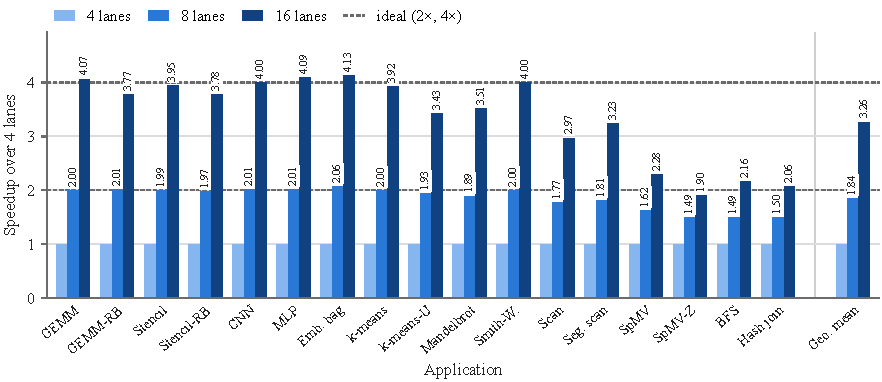
\includegraphics[width=\textwidth]{lanes_apps.pdf}\\[-1pt]
{\footnotesize (a) Applications}\\[5pt]
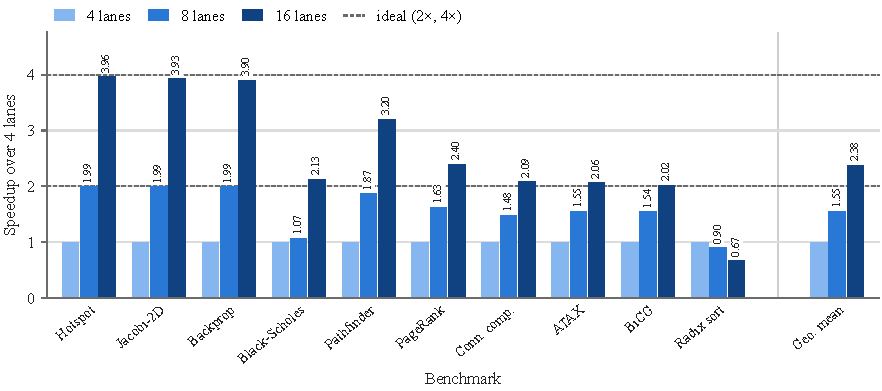
\includegraphics[width=\textwidth]{lanes_suite2.pdf}\\[-1pt]
{\footnotesize (b) Suite~2}
\caption{Speed-up over four lanes at four, eight and 16 lanes: (a) the applications,
(b) suite~2. Board-size simulation of the board configuration at each lane count
(eight warps, 16 MSHRs, 16 tags, an L1 of 2,048 lines, one divide/square-root unit
per eight lanes), board inputs, every output checked. Dashed: the ideal $2\times$ and
$4\times$. The geometric mean is over the benchmarks of the suite.}
\label{fig:lanes_suites1}
\end{figure*}

\begin{figure*}[t]
\centering
\begin{minipage}[b]{0.49\textwidth}\centering
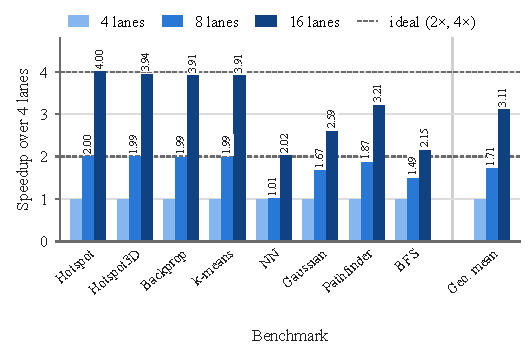
\includegraphics[width=\linewidth]{lanes_rodinia.pdf}\\[-1pt]
{\footnotesize (a) Rodinia}
\end{minipage}\hfill
\begin{minipage}[b]{0.49\textwidth}\centering
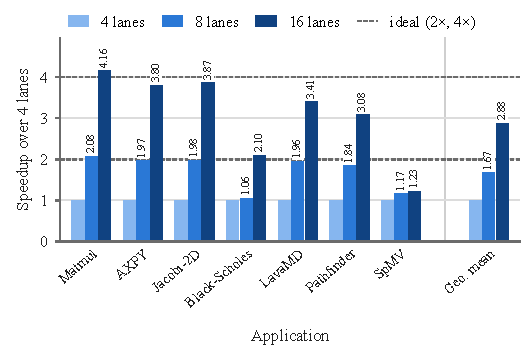
\includegraphics[width=\linewidth]{lanes_rivec.pdf}\\[-1pt]
{\footnotesize (b) RiVEC}
\end{minipage}\\[5pt]
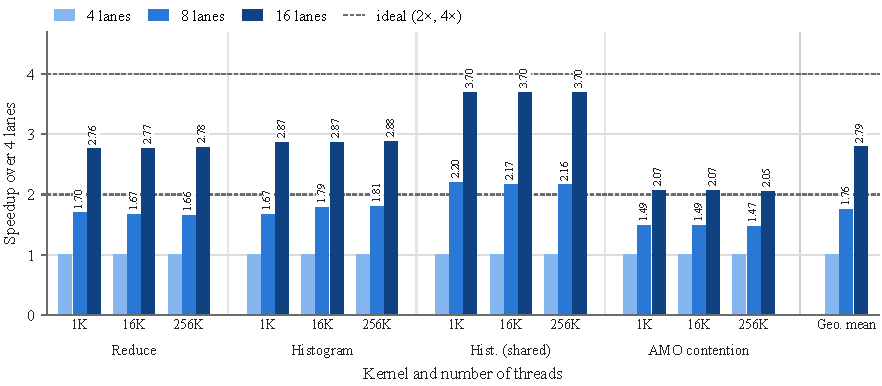
\includegraphics[width=\textwidth]{lanes_sync.pdf}\\[-1pt]
{\footnotesize (c) Synchronization kernels at 1K, 16K and 256K threads}
\caption{Speed-up over four lanes at four, eight and 16 lanes: (a) Rodinia, (b) RiVEC,
(c) the synchronization kernels, as in Fig.~\ref{fig:lanes_suites1}. At four lanes the
check of the AMO-contention kernel covers its order-independent results only (text).}
\label{fig:lanes_suites2}
\end{figure*}

Figs.~\ref{fig:lanes_suites1} and~\ref{fig:lanes_suites2} extend this comparison to
every suite we ran on the board: the 17 applications, the ten suite-2 kernels, eight
Rodinia and seven RiVEC benchmarks, and the four synchronization kernels at three
sizes, 54 cases in all. Each lane count uses its own design, with eight warps, 16
MSHRs and 16 tags throughout, an L1 of 2,048 lines (32, 64 and 128~KB), and one
divide/square-root unit per eight lanes (one at four and eight lanes, two at 16); the
eight- and 16-lane points are therefore the two board designs of
Section~\ref{sec:lanes16}. (Tables~\ref{tab:lanes_tp} and~\ref{tab:lanes_cyc} keep one
64~KB L1 and one divide/square-root unit at every lane count, so their 16-lane values
differ slightly.) We simulated each case at its board input with every output
checked, and all 54 pass at every lane count. At four lanes, the eight-thread groups of
the AMO-contention kernel span two warps whose order is not defined, so its check
covers the results that do not depend on that order: every \texttt{amoadd} sum and
every \texttt{amomax} maximum, which a lost update would change. Where the board ran
both designs, the simulated eight-to-16-lane cycle ratios agree with the measured ones
(Section~\ref{sec:lanes16}).

Over four lanes, the geometric means at eight and 16 lanes are $1.84\times$ and
$3.26\times$ for the applications, $1.55\times$ and $2.38\times$ for suite~2,
$1.71\times$ and $3.11\times$ for Rodinia, $1.67\times$ and $2.88\times$ for RiVEC, and
$1.76\times$ and $2.79\times$ for the synchronization kernels. The two groups of the
applications appear in every suite. The dense kernels (hotspot, Jacobi-2D, backprop,
hotspot3D, k-means, matmul and AXPY) come close to the ideal, with 1.97 to $2.08\times$
at eight lanes and 3.80 to $4.16\times$ at 16. The kernels that gather from large
arrays (PageRank, connected components, ATAX, BiCG, BFS and RiVEC SpMV) gain 1.17 to
$1.63\times$ and 1.23 to $2.40\times$. Three cases depart from these groups.
Black-Scholes and NN gain 1.01 to $1.07\times$ from four to eight lanes and 2.02 to
$2.13\times$ at 16, because the designs below 16 lanes have a single divide/square-root
unit. The block-shared histogram gains $2.2\times$ from four to eight lanes: at four
lanes its 32-thread blocks take all eight warps, so each block barrier stalls the whole
machine. Radix sort slows as lanes are added ($0.90\times$ and $0.67\times$), for the
line-size reason given in Section~\ref{sec:lanes16}.

The cost grows faster
than the lane count. Each lane's FPU stays at 4.8k LUTs, but the memory engine
selects the word of every lane from a line of one word per lane and places every
lane's store data into that line, and both structures grow with the square of $L$.
Section~\ref{sec:lanes16} shows that most of this growth came from one of them, the
placement of the store data, and builds the 16-lane design for the board. The 16-lane
runs also exposed the stack bound of Section~\ref{sec:arch}: in SpMV, a warp whose
rows had more than eight different lengths overflowed a stack of eight frames, and
sizing the stack by $L$ removed the failure.

\subsection{Sixteen Lanes on the Board}\label{sec:lanes16}
Tables~\ref{tab:lanes_tp} and~\ref{tab:lanes_cyc} predict that 16 lanes nearly halve
the cycles of the compute kernels. We built the 16-lane design for the ZCU102 to test
this on the board. It keeps eight warps: at the board inputs of all 42 simulated
cases (the 17 applications, ten suite-2 kernels, eight Rodinia and seven RiVEC
benchmarks), 16 lanes with four warps take only $1.25\times$ fewer cycles than the
eight-lane design, against $1.60\times$ with eight warps (geometric means), because
four warps hide too little memory latency. Three changes made the design fit the
device and use its lanes; each was simulated at board size in the exact board
configuration, with every output checked, before synthesis.

\emph{Store merging.} For a store request, the memory engine forms the data and the
byte enables of the line from the stores of the request's lanes. The original
description wrote each lane's byte, halfword or word at its offset in the line, lane
by lane, so that a higher lane overwrites a lower one at the same byte. Synthesis
builds this as one line-wide stage of shifters and multiplexers per lane, that is,
$L$ stages over $32L$ bits. Synthesized alone, with its LUTs grouped by the signal
they drive, the 16-lane engine uses 53,653 LUTs, of which 37,450 (70\%) form the
store data. The new form first replicates each lane's byte or halfword across a
32-bit word and computes its four byte enables, so that no data is shifted. Each of
the $4L$ bytes of the line then selects, with a one-hot AND-OR, the highest lane that
writes it, which keeps the overwrite order. The two forms compute the same function:
a combinational equivalence check with ABC proves it at four lanes, and random
requests ($2\times10^6$ at four and at eight lanes, $10^6$ at 16; 46 to 74\% of them
with several lanes on one word) show no difference. The store logic falls to 11,047 LUTs at 16 lanes
(3,161 at eight lanes, from 8,488) and the engine to 29,159 LUTs ($-46\%$). The
change is combinational, so no cycle count changes.

\emph{Division and square root.} One serial divide/square-root unit serves the
lanes of a warp one after another (Section~\ref{sec:arch}), so its throughput does
not grow with $L$. The 16-lane design has one unit per eight lanes; the two units
work on their halves of the warp in parallel. Each unit uses 738 LUTs. Black-Scholes
and NN, which divide or take square roots in every thread, go from $1.00$--$1.02\times$
to $2.00\times$ fewer cycles than at eight lanes.

\emph{L1 capacity.} A line holds one word per lane, so a 64~KB L1 holds 2,048 lines
at eight lanes but 1,024 lines of 64 bytes at 16. The 16-lane design uses 128~KB,
which restores 2,048 lines. The L1's data array is $32L = 512$ bits wide and already
occupies 32 RAMB36 tiles at 64~KB, eight per way for the width; the doubled depth
fills these tiles, so the larger L1 costs no block RAM, only 256 more LUTRAMs for the
tags and 1,006 flip-flops for the valid bits. It gains up to 21\% on gathers that
reuse lines (RiVEC SpMV, ATAX, BiCG, PageRank) and slows no case by more than 1\%. With both changes
the simulated speed-up over eight lanes rises from $1.60\times$ to $1.71\times$.

\begin{table}[t]
\caption{Eight- and Sixteen-Lane Board Designs on the XCZU9EG-2}
\label{tab:lanes16_impl}
\centering\footnotesize
\setlength{\tabcolsep}{4pt}
\begin{tabular}{lrr}
\toprule
 & 8 lanes & 16 lanes\\
\midrule
Clock (MHz)               & 115.37 & 100.00\\
Worst setup slack (ns)    & $+0.406$ & $+0.041$\\
\Fmax\ (MHz)              & 121.0 & 100.4\\
LUT                       & 107,658 (39\%) & 202,660 (74\%)\\
FF                        & 50,091 & 93,351\\
BRAM (RAMB36) / DSP       & 16 / 72 & 32 / 144\\
L1 size, line             & 64~KB, 32~B & 128~KB, 64~B\\
Divide/square-root units  & 1 & 2\\
Accelerator power (W)$^a$ & 1.08 & 1.79\\
\bottomrule
\end{tabular}

\vspace{2pt}
\begin{minipage}{\columnwidth}\footnotesize
Both: eight warps, 16 MSHRs, 16 tags, serial line-aggregated AMOs; complete board
designs, routed. $^a$Vivado's estimate for the accelerator; the PS adds 2.74~W in
both designs.
\end{minipage}
\end{table}

Table~\ref{tab:lanes16_impl} compares the two board designs. The 16-lane design
closes at 100~MHz, 13\% below the eight-lane clock, with 74\% of the LUTs and 96\% of
the configurable logic blocks in use; its worst path runs from a memory context's
completion flag to the write enable of the scratchpad. Before the board run we
simulated the routed netlist of the accelerator under the board-top testbench. Its
reduction, histogram and stale-line tests pass with the same cycle counts as the RTL
(1,779, 1,806 and 1,783 cycles). In the routed design, Vivado ties the constant
outputs of the accelerator's AXI4 master (burst length, size, type, cache and
protection fields, and the write ID) at the inputs of the PS port, so the netlist of
the accelerator alone leaves them undriven; we read the tied values from the routed
design and drive them in the test.

% generated by sim/compare_board_l16.py from the board logs (2026-11-17); \input where needed
\begin{table}[t]
\caption{Sixteen Lanes Against Eight Lanes and the Cortex-A53}
\label{tab:lanes16_board}
\centering\footnotesize
\setlength{\tabcolsep}{3pt}
\begin{tabular}{lrrrrr}
\toprule
 & \multicolumn{2}{c}{16 vs 8 lanes} & \multicolumn{3}{c}{vs Cortex-A53}\\
\cmidrule(lr){2-3}\cmidrule(lr){4-6}
Suite (rows) & speedup & faster & 8L & 16L & faster\\
\midrule
Sync kernels (12) & 1.34$\times$ & 12/12 & 0.17$\times$ & 0.23$\times$ & 0$\to$0\\
Applications (34) & 1.55$\times$ & 34/34 & 0.79$\times$ & 1.23$\times$ & 15$\to$19\\
Suite 2 (20) & 1.26$\times$ & 14/20 & 0.56$\times$ & 0.71$\times$ & 2$\to$6\\
Rodinia (9) & 1.64$\times$ & 9/9 & 0.56$\times$ & 0.92$\times$ & 1$\to$6\\
RiVEC (7) & 1.57$\times$ & 6/7 & 0.88$\times$ & 1.37$\times$ & 2$\to$3\\
\midrule
\textbf{All} (82) & 1.45$\times$ & 75/82 & 0.56$\times$ & 0.82$\times$ & 20$\to$34\\
\bottomrule
\end{tabular}

\end{table}


\begin{figure*}[t]
\centering
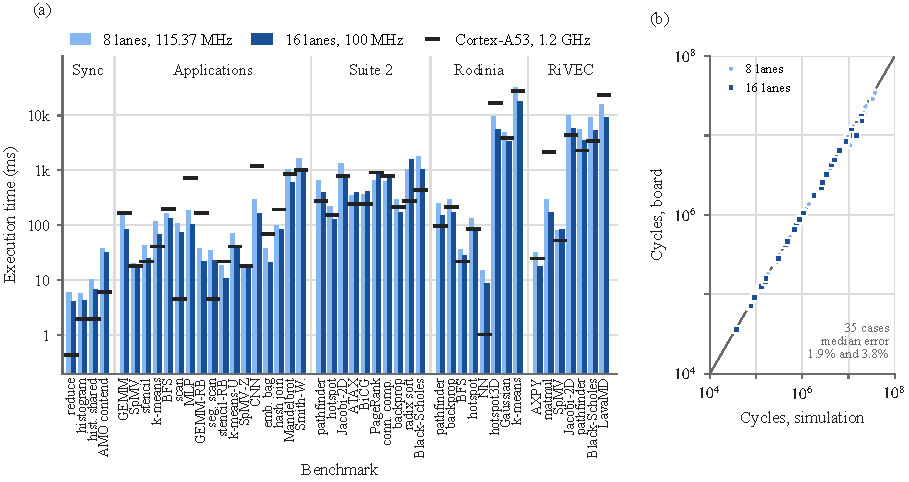
\includegraphics[width=\textwidth]{lanes16_board.pdf}
\caption{Sixteen lanes at 100~MHz against eight lanes at 115.37~MHz on the ZCU102.
(a)~Measured speed-up for each benchmark at its largest input (bars: time, which
includes the lower clock; markers: cycles). The geometric means are over all inputs
of each suite. (b)~Ratio of eight-lane to 16-lane cycles predicted by the board-size
simulation of Tables~\ref{tab:lanes_tp} and~\ref{tab:lanes_cyc} against the ratio
measured on the board, for the 42 simulated cases (hollow: the board ran more
iterations of the same kernel than the simulation).}
\label{fig:lanes16_board}
\end{figure*}

Table~\ref{tab:lanes16_board} and Fig.~\ref{fig:lanes16_board} give the board results.
We ran the same host programs and inputs as for the eight-lane design (the
synchronization kernels, the applications and suite~2 at two input sizes each, the
Rodinia and the RiVEC benchmarks), 82 runs in all; the A53 checked every output and
all pass. Over the 82 runs, the 16-lane design at 100~MHz is $1.45\times$ faster than
the eight-lane design at 115.37~MHz (geometric mean) and faster on 75. The compute
kernels of Section~\ref{sec:evallanes} take $1.91$ to $2.08\times$ fewer cycles, which
is $1.65$ to $1.80\times$ less time at the lower clock; the gather kernels (SpMV,
SpMV-Z, BFS and hash join) take $1.21$ to $1.46\times$ fewer cycles.
Against the Cortex-A53, the geometric mean rises from $0.56\times$ to $0.82\times$, and
the number of runs in which SIMTiX is faster rises from 20 to 34, among them RiVEC
matmul ($12.5\times$), GEMM-RB ($7.7\times$), the CNN ($7.1\times$), the MLP
($7.0\times$) and hotspot3D ($3.0\times$). Per run, the supplement lists all 82.

The board-size simulation predicted these results. For the 42 simulated cases, the
cycle ratio measured on the board differs from the simulated one by 1.0\% in the median
(Fig.~\ref{fig:lanes16_board}(b)); 34 cases lie within 5\%, seven are faster on the
board than predicted (by up to 15\%) and one is slower (by 7.7\%). We attribute these
differences to the board's DDR4, whose latency differs from the fixed 24 cycles of the
memory model.

Seven runs are slower at 16 lanes, with $0.65$ to $0.94\times$ the speed: radix sort
at both sizes, the larger inputs of ATAX, BiCG, PageRank and connected components, and
RiVEC SpMV. Their cycle ratios are 0.75 to 1.09, so the lower clock decides. All of
them scatter their accesses: radix sort writes each key to its bucket, and the others
gather from large arrays. Each line transfer moves 64 bytes at 16 lanes against 32 at
eight, so a scattered access moves twice the bytes for the same useful word, and the
large inputs no longer fit the L1. The smaller inputs of the same four suite-2 kernels
run $1.06$ to $1.39\times$ faster. A line size independent of the lane count, with
two requests for a full-width access, would remove this cost.

The 16-lane accelerator draws 1.79~W, against 1.08~W (Table~\ref{tab:lanes16_impl}).
With the measured speed-up, it uses 14\% more energy per run than the eight-lane
accelerator (geometric mean); counting the PS, which draws the same 2.74~W in both
designs, the system uses 18\% less.

%==============================================================================
\section{Limitations}\label{sec:disc}
%==============================================================================
SIMTiX trades frequency for IPC. Its two-stage pipeline reads the LUTRAM RFs and
decodes in the issue cycle, and its critical paths are in the lane FPUs and the
issue logic; Vortex's deeper pipeline closes at a higher frequency but needs more
warps to fill. Division and square root pass lane by lane through one shared unit
(one per eight lanes in the 16-lane design), which makes SIMTiX slower than Ara and
Vortex on nn and blackscholes, and divergent code leaves lanes idle. One Cortex-A53
core at 1.2~GHz, 10.4 times SIMTiX's clock, remains faster than the eight-lane
SIMTiX on 12 of the 15 Rodinia and RiVEC benchmarks, and faster than the 16-lane
design on 7 of the 16 Rodinia and RiVEC runs. The L1 line holds one word per lane,
so at 16 lanes every line transfer moves 64 bytes; kernels that scatter their
accesses over large arrays then move twice the bytes per useful word and run slower
than at eight lanes (Section~\ref{sec:lanes16}).

SIMTiX has no compiler: its kernels are hand-written assembly, while Vortex's are
compiled by LLVM, so part of Vortex's larger instruction count reflects compiled code
rather than the instruction set; the efficiency factor of Section~\ref{sec:decomp}
includes both. Ara runs RiVEC's own vector code, changed in two places to avoid
faults of Ara (Section~\ref{sec:rivec}). Power was measured on the board for SIMTiX
and the A53 only; the out-of-context comparison with Vortex uses vectorless
estimates. All machines were evaluated as single cores; multi-core configurations,
which Vortex supports with an L2 cache and an OpenCL stack, were not. The AMOs exclude
load-reserved and store-conditional.

%==============================================================================
\section{Conclusion}
%==============================================================================
This paper presented SIMTiX, a SIMT accelerator of eight lanes and eight warps for
FPGA systems-on-chip, and measured it against a scalar, a vector and a SIMT RISC-V
machine on the same ZCU102. Its issue logic hides latency with few warps: pipelined
units, a register scoreboard with sleeping warps, non-blocking loads, eight warps and
a memory system with 16 requests in flight together gain $1.68\times$ over our earlier
design without changing an instruction. Its memory engine sends one request per line
touched and keeps up to 16 in flight, against one miss for CVA6 and four elements of a
strided or indexed access for Ara. Line-aggregated AMOs serve all lanes of an atomic
that share a line with one read and one write while preserving the results of serial
execution, for 660 LUTs. The complete board design uses 107,658 LUTs and closes at
115.4~MHz. On 15 Rodinia and RiVEC benchmarks SIMTiX is $16.9\times$, $3.1\times$ and
$2.5\times$ faster than CVA6, Ara and Vortex. Splitting these ratios into clock, width
and efficiency shows that SIMTiX leads Ara through its width and, on irregular
accesses, its memory-level parallelism, and leads Vortex through efficiency alone.
A 16-lane version, in which a restructured store merge shrinks the memory engine by
46\%, closes at 100~MHz and runs 82 benchmark runs $1.45\times$ faster than
the eight-lane design, as its board-size simulation predicted. Its remaining limits
are division and square root, divergent code, and, at 16 lanes, a line size tied to
the lane count. A divide pipelined through the FMA units and a line size independent
of the lane count are the next steps.

%==============================================================================
\section*{Acknowledgment}
%==============================================================================
The authors used a large language model (Anthropic Claude) to assist with build
and analysis scripting and with editing this manuscript. The design, the
experiments and their interpretation are the authors' own, and the authors checked
every reported result.

%==============================================================================
\begin{thebibliography}{99}
\bibitem{tesla} E.~Lindholm, J.~Nickolls, S.~Oberman, and J.~Montrym,
``NVIDIA Tesla: A unified graphics and computing architecture,''
\emph{IEEE Micro}, vol.~28, no.~2, pp.~39--55, Mar. 2008.
\bibitem{aamodt} T.~M.~Aamodt, W.~W.~L.~Fung, and T.~G.~Rogers,
\emph{General-Purpose Graphics Processor Architectures}. San Rafael, CA, USA:
Morgan \& Claypool, 2018.
\bibitem{vortex} B.~Tine, K.~P.~Yalamarthy, F.~Elsabbagh, and H.~Kim,
``Vortex: Extending the RISC-V ISA for GPGPU and 3D-graphics,'' in
\emph{Proc. IEEE/ACM Int. Symp. Microarchitecture (MICRO)}, 2021, pp.~754--766.
\bibitem{ventus25} J.~Li \emph{et al.}, ``RISC-V-based GPGPU with vector
capabilities for high-performance computing,'' \emph{IEEE Trans. Very Large Scale
Integr. (VLSI) Syst.}, vol.~33, no.~8, pp.~2239--2252, Aug. 2025.
\bibitem{egpu} M.~Langhammer and G.~A.~Constantinides, ``eGPU: A 750 MHz class
soft GPGPU for FPGA,'' in \emph{Proc. Int. Conf. Field-Programmable Logic Appl.
(FPL)}, 2023.
\bibitem{flexgrip} K.~Andryc, M.~Merchant, and R.~Tessier, ``FlexGrip: A soft
GPGPU for FPGAs,'' in \emph{Proc. Int. Conf. Field-Programmable Technol. (FPT)},
2013.
\bibitem{fgpu} M.~Al~Kadi, B.~Janssen, and M.~H\"ubner, ``FGPU: An
SIMT-architecture for FPGAs,'' in \emph{Proc. ACM/SIGDA Int. Symp.
Field-Programmable Gate Arrays (FPGA)}, 2016, pp.~254--263.
\bibitem{miaow} R.~Balasubramanian \emph{et al.}, ``Enabling GPGPU low-level
hardware explorations with MIAOW: An open-source RTL implementation of a GPGPU,''
\emph{ACM Trans. Archit. Code Optim.}, vol.~12, no.~2, 2015.
\bibitem{nyuzi} J.~Bush, P.~Dexter, T.~N.~Miller, and A.~Carpenter, ``Nyami: A
synthesizable GPU architectural model for general-purpose and graphics-specific
workloads,'' in \emph{Proc. IEEE Int. Symp. Perform. Anal. Syst. Softw.
(ISPASS)}, 2015.
\bibitem{simty} S.~Collange, ``Simty: Generalized SIMT execution on RISC-V,'' in
\emph{Proc. Workshop Comput. Archit. Res. RISC-V (CARRV)}, 2017.
\bibitem{fung} W.~W.~L.~Fung, I.~Sham, G.~Yuan, and T.~M.~Aamodt, ``Dynamic warp
formation and scheduling for efficient GPU control flow,'' in \emph{Proc. IEEE/ACM
Int. Symp. Microarchitecture (MICRO)}, 2007, pp.~407--420.
\bibitem{fermi} NVIDIA, ``NVIDIA's next generation CUDA compute architecture:
Fermi,'' White Paper, 2009.
\bibitem{dab} Y.~H.~Chou, C.~Ng, S.~Cattell, J.~Intan, M.~D.~Sinclair,
J.~Devietti, T.~G.~Rogers, and T.~M.~Aamodt, ``Deterministic atomic buffering,''
in \emph{Proc. IEEE/ACM Int. Symp. Microarchitecture (MICRO)}, 2020,
pp.~981--995.
\bibitem{franey} S.~Franey and M.~Lipasti, ``Accelerating atomic operations on
GPGPUs,'' in \emph{Proc. IEEE/ACM Int. Symp. Networks-on-Chip (NOCS)}, 2013,
pp.~1--8.
\bibitem{phi} A.~Mukkara, N.~Beckmann, and D.~Sanchez, ``PHI: Architectural
support for synchronization- and bandwidth-efficient commutative scatter
updates,'' in \emph{Proc. IEEE/ACM Int. Symp. Microarchitecture (MICRO)}, 2019,
pp.~1009--1022.
\bibitem{warpagg} A.~Adinets, ``CUDA pro tip: Optimized filtering with
warp-aggregated atomics,'' NVIDIA Developer Blog, Oct. 2014.
\bibitem{axi} Arm Ltd., \emph{AMBA AXI and ACE Protocol Specification}, ARM IHI
0022E, 2013.
\bibitem{boldo} S.~Boldo and G.~Melquiond, ``Emulation of FMA and correctly rounded
sums: Proved algorithms using rounding to odd,'' \emph{IEEE Trans. Comput.}, vol.~57,
no.~4, pp.~462--471, Apr. 2008.
\bibitem{figueroa} S.~A.~Figueroa, ``When is double rounding innocuous?''
\emph{ACM SIGNUM Newsl.}, vol.~30, no.~3, pp.~21--26, 1995.
\bibitem{ieee754} \emph{IEEE Standard for Floating-Point Arithmetic}, IEEE Std
754-2019, 2019.
\bibitem{rodinia} S.~Che, M.~Boyer, J.~Meng, D.~Tarjan, J.~W.~Sheaffer, S.-H.~Lee,
and K.~Skadron, ``Rodinia: A benchmark suite for heterogeneous computing,'' in
\emph{Proc. IEEE Int. Symp. Workload Characterization (IISWC)}, 2009, pp.~44--54.
\bibitem{gap} S.~Beamer, K.~Asanovi\'c, and D.~Patterson, ``The GAP benchmark suite,''
arXiv:1508.03619, 2015.
\bibitem{shoc} A.~Danalis, G.~Marin, C.~McCurdy, J.~S.~Meredith, P.~C.~Roth, K.~Spafford,
V.~Tipparaju, and J.~S.~Vetter, ``The Scalable Heterogeneous Computing (SHOC) benchmark
suite,'' in \emph{Proc. 3rd Workshop General-Purpose Comput. Graph. Process. Units
(GPGPU-3)}, 2010, pp.~63--74.
\bibitem{polybench} L.-N.~Pouchet, ``PolyBench/C: The polyhedral benchmark suite,''
2012. [Online]. Available: \url{https://sourceforge.net/projects/polybench/}
% TO CHECK: article number and pages of rivec (ACM TACO 17(4), 2020)
\bibitem{rivec} C.~Ram\'{\i}rez, C.~A.~Hern\'andez, O.~Palomar, O.~Unsal,
M.~A.~Ram\'{\i}rez, and A.~Cristal, ``A RISC-V simulator and benchmark suite for
designing and evaluating vector architectures,'' \emph{ACM Trans. Archit. Code
Optim.}, vol.~17, no.~4, Art.~38, Dec. 2020.
% TO CHECK on IEEE Xplore: volume, number and pages of ara, ara2 and cva6
\bibitem{ara} M.~Cavalcante, F.~Schuiki, F.~Zaruba, M.~Schaffner, and L.~Benini,
``Ara: A 1-GHz+ scalable and energy-efficient RISC-V vector processor with
multiprecision floating-point support in 22-nm FD-SOI,'' \emph{IEEE Trans. Very Large
Scale Integr. (VLSI) Syst.}, vol.~28, no.~2, pp.~530--543, Feb. 2020.
\bibitem{ara2} M.~Perotti, M.~Cavalcante, R.~Andri, L.~Cavigelli, and L.~Benini,
``Ara2: Exploring single- and multi-core vector processing with an efficient RVV~1.0
compliant open-source processor,'' \emph{IEEE Trans. Comput.}, 2024.
\bibitem{cva6} F.~Zaruba and L.~Benini, ``The cost of application-class processing:
Energy and performance analysis of a Linux-ready 1.7-GHz 64-bit RISC-V core in 22-nm
FDSOI technology,'' \emph{IEEE Trans. Very Large Scale Integr. (VLSI) Syst.},
vol.~27, no.~11, 2019.
\end{thebibliography}

\end{document}
